\documentclass[leqno, openany]{memoir}
\setulmarginsandblock{3.5cm}{3.5cm}{*}
\setlrmarginsandblock{3cm}{3.5cm}{*}
\checkandfixthelayout

\usepackage{amsmath}
\usepackage{amssymb}
\usepackage{amsthm}
%\usepackage{MnSymbol}
\usepackage{bm}
\usepackage{accents}
\usepackage{mathtools}
\usepackage{tikz}
\usetikzlibrary{decorations.pathmorphing,shapes}
\usetikzlibrary{calc}
\usetikzlibrary{automata,positioning}
\usepackage{tikz-cd}
\usepackage{forest}
\usepackage{braket} 
\usepackage{listings}
\usepackage{mdframed}
\usepackage{verbatim}
\usepackage{physics}
\usepackage{stmaryrd}
\usepackage{mathrsfs} 
\usepackage{stackengine} 
%\usepackage{/home/patrickl/homework/macaulay2}

%font
\usepackage[sc]{mathpazo}
\usepackage{eulervm}
\usepackage[scaled=0.86]{berasans}
\usepackage{inconsolata}
\usepackage{microtype}

%CS packages
\usepackage{algorithmicx}
\usepackage{algpseudocode}
\usepackage{algorithm}

% typeset and bib
\usepackage[english]{babel} 
\usepackage[utf8]{inputenc} 
\usepackage[T1]{fontenc}
\usepackage[backend=biber, style=alphabetic]{biblatex}
\usepackage[bookmarks, colorlinks, breaklinks]{hyperref} 
\hypersetup{linkcolor=black,citecolor=black,filecolor=black,urlcolor=black}

% other formatting packages
\usepackage{float}
\usepackage{booktabs}
\usepackage[shortlabels]{enumitem}
\usepackage{csquotes}
\usepackage{titlesec}
\usepackage{titling}
\usepackage{fancyhdr}
\usepackage{lastpage}
\usepackage{parskip}
\usepackage{graphicx}
\graphicspath{{./images/}}

\usepackage{lipsum}

% delimiters
\DeclarePairedDelimiter{\gen}{\langle}{\rangle}
\DeclarePairedDelimiter{\floor}{\lfloor}{\rfloor}
\DeclarePairedDelimiter{\ceil}{\lceil}{\rceil}


\newtheorem{thm}{Theorem}[section]
\newtheorem{cor}[thm]{Corollary}
\newtheorem{prop}[thm]{Proposition}
\newtheorem{lem}[thm]{Lemma}
\newtheorem{conj}[thm]{Conjecture}
\newtheorem{quest}[thm]{Question}

\theoremstyle{definition}
\newtheorem{defn}[thm]{Definition}
\newtheorem{defns}[thm]{Definitions}
\newtheorem{con}[thm]{Construction}
\newtheorem{exm}[thm]{Example}
\newtheorem{exms}[thm]{Examples}
\newtheorem{notn}[thm]{Notation}
\newtheorem{notns}[thm]{Notations}
\newtheorem{addm}[thm]{Addendum}
\newtheorem{exer}[thm]{Exercise}

\theoremstyle{remark}
\newtheorem{rmk}[thm]{Remark}
\newtheorem{rmks}[thm]{Remarks}
\newtheorem{warn}[thm]{Warning}
\newtheorem{sch}[thm]{Scholium}


% unnumbered theorems
\theoremstyle{plain}
\newtheorem*{thm*}{Theorem}
\newtheorem*{prop*}{Proposition}
\newtheorem*{lem*}{Lemma}
\newtheorem*{cor*}{Corollary}
\newtheorem*{conj*}{Conjecture}

% unnumbered definitions
\theoremstyle{definition}
\newtheorem*{defn*}{Definition}
\newtheorem*{exer*}{Exercise}
\newtheorem*{defns*}{Definitions}
\newtheorem*{con*}{Construction}
\newtheorem*{exm*}{Example}
\newtheorem*{exms*}{Examples}
\newtheorem*{notn*}{Notation}
\newtheorem*{notns*}{Notations}
\newtheorem*{addm*}{Addendum}


\theoremstyle{remark}
\newtheorem*{rmk*}{Remark}

% shortcuts
\newcommand{\Ima}{\mathrm{Im}}
\newcommand{\A}{\mathbb{A}}
\newcommand{\G}{\mathbb{G}}
\newcommand{\N}{\mathbb{N}}
\newcommand{\R}{\mathbb{R}}
\newcommand{\C}{\mathbb{C}}
\newcommand{\Z}{\mathbb{Z}}
\newcommand{\Q}{\mathbb{Q}}
\newcommand{\U}{\mathcal{U}}
\newcommand{\cO}{\mathcal{O}}
\renewcommand{\k}{\Bbbk}
\renewcommand{\P}{\mathbb{P}}
\newcommand{\M}{\overline{M}}
\newcommand{\g}{\mathfrak{g}}
\newcommand{\h}{\mathfrak{h}}
\newcommand{\n}{\mathfrak{n}}
\renewcommand{\b}{\mathfrak{b}}
\newcommand{\ep}{\varepsilon}
\newcommand*{\dt}[1]{%
   \accentset{\mbox{\Huge\bfseries .}}{#1}}
\renewcommand{\abstractname}{Official Description}
\newcommand{\mc}[1]{\mathcal{#1}}
\newcommand{\T}{\mathbb{T}}
\newcommand{\mf}[1]{\mathfrak{#1}}
\newcommand{\mr}[1]{\mathrm{#1}}
\newcommand{\on}[1]{\operatorname{#1}}
\newcommand{\ms}[1]{\mathsf{#1}}
\newcommand{\ol}[1]{\overline{#1}}
\newcommand{\ul}[1]{\underline{#1}}
\newcommand{\wt}[1]{\widetilde{#1}}
\newcommand{\wh}[1]{\widehat{#1}}
\renewcommand{\div}{\operatorname{div}}
\newcommand{\Sm}{\mathsf{Sm}}
\newcommand{\Cor}{\mathsf{Cor}}

\DeclareMathOperator{\Der}{Der}
\DeclareMathOperator{\Hom}{Hom}
\DeclareMathOperator{\End}{End}
\DeclareMathOperator{\Ext}{Ext}
\DeclareMathOperator{\ext}{ext}
\DeclareMathOperator{\ad}{ad}
\DeclareMathOperator{\Aut}{Aut}
\DeclareMathOperator{\Rad}{Rad}
\DeclareMathOperator{\Pic}{Pic}
\DeclareMathOperator{\supp}{supp}
\DeclareMathOperator{\Supp}{Supp}
\DeclareMathOperator{\sgn}{sgn}
\DeclareMathOperator{\spec}{Spec}
\DeclareMathOperator{\rk}{rk}
\DeclareMathOperator{\Spec}{Spec}
\DeclareMathOperator{\proj}{Proj}
\DeclareMathOperator{\Proj}{Proj}
\DeclareMathOperator{\ord}{ord}
\DeclareMathOperator{\Div}{Div}
\DeclareMathOperator{\Bl}{Bl}
\DeclareMathOperator{\ch}{ch}
\DeclareMathOperator{\td}{td}
\DeclareMathOperator{\Tor}{Tor}
\DeclareMathOperator{\depth}{depth}
\DeclareMathOperator{\CH}{CH}
\DeclareMathOperator{\Ob}{Ob}
\DeclareMathOperator{\Rat}{Rat} 
\DeclareMathOperator{\coker}{coker}
\DeclareMathOperator{\Hilb}{Hilb}
\DeclareMathOperator{\Sym}{Sym}
\DeclareMathOperator{\Conn}{\ms{Conn}}
\DeclareMathOperator{\Loc}{\ms{Loc}}
\DeclareMathOperator{\Perv}{\ms{Perv}}
\DeclareMathOperator{\Mod}{\ms{Mod}}
\DeclareMathOperator{\gr}{gr}
\DeclareMathOperator{\Ch}{Ch}
\DeclareMathOperator{\CC}{CC}
\DeclareMathOperator{\mult}{mult}
\DeclareMathOperator{\reg}{reg}
\DeclareMathOperator{\Tot}{Tot}
\DeclareMathOperator{\Sol}{Sol}

\makeatletter
\DeclareRobustCommand\widecheck[1]{{\mathpalette\@widecheck{#1}}}
\def\@widecheck#1#2{%
    \setbox\z@\hbox{\m@th$#1#2$}%
    \setbox\tw@\hbox{\m@th$#1%
       \widehat{%
          \vrule\@width\z@\@height\ht\z@
          \vrule\@height\z@\@width\wd\z@}$}%
    \dp\tw@-\ht\z@
    \@tempdima\ht\z@ \advance\@tempdima2\ht\tw@ \divide\@tempdima\thr@@
    \setbox\tw@\hbox{%
       \raise\@tempdima\hbox{\scalebox{1}[-1]{\lower\@tempdima\box
\tw@}}}%
    {\ooalign{\box\tw@ \cr \box\z@}}}
\makeatother

% Section formatting
\titleformat{\section}
    {\Large\sffamily\scshape\bfseries}{\thesection}{1em}{}
\titleformat{\subsection}[runin]
    {\large\sffamily\bfseries}{\thesubsection}{1em}{}
\titleformat{\subsubsection}[runin]{\normalfont\itshape}{\thesubsubsection}{1em}{}

\title{COURSE TITLE}
\author{Lectures by INSTRUCTOR, Notes by NOTETAKER}
\date{SEMESTER}

\newcommand*{\titleSW}
    {\begingroup% Story of Writing
    \raggedleft
    \vspace*{\baselineskip}
    {\Huge\itshape Geometric Representation Theory Learning Seminar \\ Spring 2022}\\[\baselineskip]
    {\large\itshape Notes by Patrick Lei}\\[0.2\textheight]
    {\Large Lectures by Various}\par
    \vfill
    {\Large \sffamily Columbia University}
    \vspace*{\baselineskip}
\endgroup}
\pagestyle{simple}

\chapterstyle{ell}


%\renewcommand{\cftchapterpagefont}{}
\renewcommand\cftchapterfont{\sffamily}
\renewcommand\cftsectionfont{\scshape}
\renewcommand*{\cftchapterleader}{}
\renewcommand*{\cftsectionleader}{}
\renewcommand*{\cftsubsectionleader}{}
\renewcommand*{\cftchapterformatpnum}[1]{~\textbullet~#1}
\renewcommand*{\cftsectionformatpnum}[1]{~\textbullet~#1}
\renewcommand*{\cftsubsectionformatpnum}[1]{~\textbullet~#1}
\renewcommand{\cftchapterafterpnum}{\cftparfillskip}
\renewcommand{\cftsectionafterpnum}{\cftparfillskip}
\renewcommand{\cftsubsectionafterpnum}{\cftparfillskip}
\setrmarg{3.55em plus 1fil}
\setsecnumdepth{subsection}
\maxsecnumdepth{subsection}
\settocdepth{subsection}

\begin{document}
    
\begin{titlingpage}
\titleSW
\end{titlingpage}

\thispagestyle{empty}
\section*{Disclaimer}%
\label{sec:disclaimer}

These notes were taken during the seminar using the \texttt{vimtex} package of
the editor \texttt{neovim}.  Any errors are mine and not the speakers'.  In
addition, my notes are picture-free (but will include commutative diagrams) and
are a mix of my mathematical style and that of the lecturers.  If you find any
errors, please contact me at \texttt{plei@math.columbia.edu}.

\vspace*{1cm}

\noindent\textbf{Seminar Website:}\\
\url{https://math.columbia.edu/~plei/s22-GRT.html} \newpage

\tableofcontents

\chapter{Fan (Feb 09): D-modules, bare minimumz, part 1}%

For now, let $X = \Spec A$ be a smooth affine variety over $\C$.

\begin{defn}
    A \textit{differential operator of order $\leq i$} is a $\C$-linear $D \colon A \to A$ such that for any $\phi \in A$, $[D, \phi]$ is a differential operator of order $\leq i-1$. In other words, for any $\phi_0, \ldots, \phi_n \in A$, we have
    \[ [\phi_n, \ldots, [\phi_2, [\phi_1, [\phi_0, D]]]] = 0. \]
\end{defn}
We will call the set of differential operators of order $\leq i$ $\mc{D}^i$. We will see later that $\mc{O}_X \cong \mc{D}^0$, $\mc{O}_X \oplus \mc{T}_X \cong \mc{D}^1$, and $\on{Gr}^i \mc{D} \cong \on{Sym}_{\mc{O}_X}^i \mc{T}_X$. Some other facts are:
\begin{itemize}
    \item $\mc{D}$ is generated by $\mc{O}_X, \mc{T}_X$ under the rules
        \[ \phi_1 * \phi_2 = \phi_1 \phi_2 \qquad \phi * \xi = \phi \xi \qquad \xi_1 * \xi_2 - \xi_2 * \xi_1 = [\xi_1, \xi_2] \qquad \xi * \phi - \phi * \xi = \xi(\phi). \]
    \item For any $\phi \in A$, $A_{\phi} \otimes_A \mc{D}^i(A) \cong D^i(A_{\phi})$.
\end{itemize}

We will now prove these facts. First, $\mc{O}_X \cong \mc{D}^1(X)$ by $\phi \mapsto \cdot \phi$ and $D \mapsto D(1)$. On the other hand, we note that $\mc{O}_X \oplus \mc{T}_X \to \mc{D}^1$ is given by $\phi \oplus \xi \mapsto (\cdot \phi) + \xi(-)$ and $D \mapsto D(1) \oplus [D,-]$.

\begin{lem}
    We have $\mc{D}^i \cdot \mc{D}^j \subseteq \mc{D}^{i+j}$ and $[\mc{D}^i, \mc{D}^j] \subseteq \mc{D}^{i+j-1}$.
\end{lem}

\begin{prop}
    There is a canonical map $\on{Sym}_{\mc{O}_X} \mc{T}_X \to \mc{D}_X$.
\end{prop}

On one hand, note that $\mc{T}_X \simeq \on{Gr}^1(D)$. Taking symmetric powers of this, we obtain a map $\on{Sym} \mc{T}_X \to \on{Gr} \mc{D}$.

To define the inverse, note that we have a morphism in degree $0$ already. Inductively, we consider the map
\[ \mc{O}_X \otimes \mc{D}^n_X \to \on{Gr}^{n-1} \mc{D}_X \qquad \phi \otimes D \mapsto [D, \phi]. \]
This kills $\mc{O}_X \otimes \mc{D}^{n-1}_X$, so it descends to $\mc{O}_X \otimes \on{Gr}^n \mc{D}_X$. Inductively, we use the adjunction to obtain
\[ \on{Gr}^n \mc{D}_X \to \Der(\mc{O}_X, \on{Sym}_{\mc{O}_X}^{n-1} \mc{T}_X) = \ul{\Hom}_{\mc{O}_X}(\Omega_X, \on{Sym}^{n-1}_{\mc{O}_X} \mc{T}_X) = \on{Sym}^{n-1}_{\mc{O}_X} \mc{T}_X \otimes \mc{T}_X \to \on{Sym}^n \mc{T}_X. \]
It is easy to check that this is an inverse.

We will now consider generation of $\mc{D}$ by $\mc{O}$ and $\mc{T}$. We will endow $\mc{O} \oplus \mc{T}$ with the Lie bracket 
\[ \qty{\phi_1, \phi_2} = 0, \qquad \qty{\xi, \phi} = \xi(\phi), \qquad \qty{\xi_1, \xi_2} = [\xi_1, \xi_2]. \]
We will show that
\[ \mc{D}_X = \mc{U}(\mc{O}_X \oplus \mc{T}_X) / \ev{\phi_1 * \phi_2 = \phi_1 \phi_2, \phi * \xi = \phi \xi}. \]
Clearly there is a map $\phi \mapsto \phi, \xi \mapsto \xi$, whose source we call $\mc{U}$. The commutation relations imply that $\on{Gr} \mc{U}$ is commutative, so we have a surjection
\[ \on{Sym}_{\mc{O}_X} \mc{T}_x \twoheadrightarrow \on{Gr} \mc{U} \to \on{Gr} \mc{D}_X. \]
Clearly, we see that $\on{Gr} \mc{U} \to \on{D}_X$ is an isomorphism, so $\mc{U} \to \mc{D}_X$ is an isomorphism.

Finally, consider the map $A_{\phi} \otimes \mc{D}^i(A) \to \mc{D}^i(A_{\phi})$ given by
\[ \frac{\psi}{\phi^n} \otimes D \mapsto \frac{1}{\phi^n} D(\psi) - \frac{1}{\phi^n} f^{i-1} \qty(\frac{\psi}{\phi^n} \otimes [D, \phi^n]). \]
Clearly this is well-defined, so it suffices to check that $A_{\phi} \otimes \on{Gr}^i \mc{D}(A) \to \on{Gr}^i D(A_{\phi})$ is an isomorphism. But both sides are $A_{\phi} \otimes \on{Sym}^i T_A = \on{Sym}^i T_{A_{\phi}}$, and by exactness of localization we are done.

Now that we have a sheaf $\mc{D}_X$, we will define $\mc{D}_X$-modules.
\begin{defn}
    A \textit{left $\mc{D}_X$-module} is a quasicoherent sheaf with a left $\mc{D}_X$-action.
\end{defn}

\begin{exm}
    Clearly $\mc{D}_X$ and $\mc{O}_X$ are $\mc{D}_X$-modules. On the other hand, if $k_x$ is the skyscraper sheaf at $x \in X$, then $k_x \otimes \mc{D}_X$ is a right $\mc{D}_X$-module.
\end{exm}

\begin{prop}
    Let $\mc{F}, \mc{F}' \in \mc{D}_X\ms{-Mod}$. Then
    \begin{itemize}
        \item $\mc{F} \otimes \mc{F}'$ is a left $\mc{D}_X$-module with the formula
            \[ \xi(v \otimes v') = \xi v \otimes v' + v \otimes \xi v'. \]
        \item $\ul{Hom}_{\mc{O}_X}(\mc{F}, \mc{F}')$ is a left $\mc{D}_X$-module by
            \[ (\xi f)(v) = \xi(f(v)) - f(\xi(v)). \]
            The analogous statement is true for right modules.
        \item If $\mc{G}$ is a right $\mc{D}_X$-module, then $\mc{G} \otimes \mc{F}$ is a right module by
            \[ (w \otimes v) \xi = w \xi \otimes v - w \otimes \xi v. \]
        \item $\ul{\Hom}_{\mc{O}_X}(\mc{F}, \mc{G})$ is a right module by
            \[ f \xi(v) = f(v) \xi + f(\xi v). \]
    \end{itemize}
\end{prop}

Recall that $\mc{T}_X$ acts on $\Omega^n_X$ by the Lie derivative. Then $\det \Omega_X$ admits a right $\mc{D}_X$-module structure by $w \cdot \xi = - \on{Lie}_{\xi} \omega$.

\begin{defn}
    Define the right $\mc{D}_X$-module $\Omega_{\mc{D}_X}$ by
    \[ \Omega_{\mc{D}_X} \coloneqq \det \Omega_X \otimes \mc{D}_X. \]
\end{defn}

Now if $\mc{F}$ is a left $\mc{D}_X$-module, then we see that 
\[ \Omega_{\mc{D}_X} \otimes_{\mc{D}_X} \mc{F} = \det \Omega_X \otimes_{\mc{O}_X} \mc{F} \]
is a right $\mc{D}_X$-module. Now if $\mc{G}$ is a right $\mc{D}_X$-module, then
\begin{align*}
    \ul{\Hom}_{\mc{D}_X^{\mr{op}}}(\Omega_{\mc{D}_X}, \mc{G}) &\cong \ul{\Hom}_{\mc{O}_X}(\det \Omega_X, \mc{G}) \\
    &= \mc{G} \otimes \mc{O}_X (\det \Omega_X)^{\vee} \\
    &= \mc{G} \otimes_{\mc{D}_X} \ul{\Hom}_{\mc{D}_X^{\mr{op}}}(\Omega_{\mc{D}_X}, \mc{D}_X).
\end{align*}
We will call this sheaf $\Omega_{\mc{D}_X}^{\dag}$.

\begin{prop}
    The functors $\det \Omega_X \otimes_{\mc{O}_X} -$ and $\ul{\Hom}_{\mc{O}_X}(\det \Omega_X, -)$ give an equivalence of categories between $\mc{D}_X\ms{-Mod}$ and $\ms{Mod-}\mc{D}_X$.
\end{prop}

\begin{proof}
    We will prove an adjunction
    \[ \Psi \colon \Hom_{\mc{D}_X^{\mr{op}}} (\det \Omega_X \otimes -, -) \to \Hom_{\mc{D}_X}(-, \ul{\Hom}_{\mc{O}_X}(\det \Omega_X, -)). \]
    This will be defined by
    \[ \Psi f(\xi v) = \xi \Psi f(v) = \xi(\omega \mapsto f(\omega \otimes v)) = - f(\omega \otimes v) \xi + f(\xi \omega \otimes v). \]
    Here, we note that $f(\xi \omega \otimes v) - f(\omega \otimes \xi v) = f((\omega \otimes v) \xi)$, so we have the adjunction. We only need to check that the unit and counit are isomorphisms now. Here, we have
    \begin{align*}
        \det \Omega_X \otimes_{\mc{O}_X} \ul{\Hom}_{\mc{O}_X}(\det \Omega_X, \mc{F}) &= \det \Omega_X \otimes \mc{F} \otimes (\det \Omega_X)^{\vee} \\
        &= \mc{F},
    \end{align*}
    and the unit is similar.
\end{proof}

\chapter{Fan (Feb 16): D-modules, bare minimumz, part 2}%

Our goal is the following underived theorem:
\begin{thm}[Kashiwara]
    Let $\iota \colon X \to Y$ be a closed immersion. Then there exist functors
    \[\iota_+ \colon \mc{D}_X\ms{-Mod} \to \mc{D}_Y\ms{-Mod}_X, \qquad \iota^+ \colon \mc{D}_Y\ms{-Mod}_X \to \mc{D}_X\ms{-Mod} \] 
    giving an equivalence of categories.
\end{thm}

\begin{defn}
    Let $f \colon X \to Y$ be a morphism. Then the $\mc{D}$-module pullback $f^*$ is defined by
    \[ f^* \mc{F} = \mc{O}_X \otimes_{f^{-1} \mc{O}_Y} f^{-1} \mc{F} \]
    with the $\mc{D}_X$-action given by 
    \[ \xi(\phi \otimes v) = \xi(\phi) v + \phi \dd{f}(\xi) v. \]
\end{defn}

\section{Transfer modules}

\begin{defn}
    Define the \textit{transfer module} $\mc{D}_{X \to Y} \coloneqq f^* \mc{D}_Y$.
\end{defn}

Now that we have this definition, it is clear that $f^* \mc{F} = \mc{D}_{X \to Y} \otimes_{f^{-1} \mc{D}_Y} f^{-1} \mc{F}$.

\begin{defn}
    Define the functor $f_+ \colon \mc{D}_X\ms{-Mod} \to \mc{D}_Y\ms{-Mod}$ by
    \[ f_+ \mc{F} = \ul{\Hom}_{\mc{D}_Y^{\mr{op}}}(\Omega_{\mc{D}_Y}, f_* ( \Omega_{\mc{D}_X} \otimes_{\mc{D}_X} \mc{F} \otimes_{\mc{D}_X} \mc{D}_{X \to Y} ) ). \]
\end{defn}

After symbol pushing, we obtain
\begin{align*}
    f_+ \mc{F} &= \ul{\Hom}_{\mc{O}_Y}(\det \Omega_Y, f_* (\det \Omega_X) \otimes_{\mc{O}_X} \mc{F} \otimes_{\mc{D}_X} \mc{D}_{X \to Y}) \\
    &= \ul{\Hom}_{\mc{O}_Y} (\det \Omega_Y, f_*(\det \Omega_X \otimes_{\mc{O}_X} \mc{D}_{X \to Y} \otimes_{\mc{D}_X} \mc{F})) \\
    &= f_* \ul{\Hom}_{\mc{O}_X} (f^* \det \Omega_Y, \det \Omega_X \otimes_{\mc{O}_X} \mc{D}_{X \to Y} \otimes_{\mc{D}_X} \mc{F}) \\
    &= f_* \qty((\det \Omega_X) \otimes_{\mc{O}_X} \mc{D}_{X \to Y} \otimes_{\mc{D}_X} \mc{F} \otimes_{\mc{O}_X} f^* \det \Omega_Y^*) \\
    &= f_* ((\det \Omega_X \otimes_{\mc{O}_X} \mc{D}_{X \to Y}) \otimes_{\mc{D}_X} (\mc{F} \otimes_{\mc{O}_X} f^* \det \Omega_Y^*)) \\
    &= f_* (\det \Omega_X \otimes_{\mc{O}_X} \mc{D}_{X \to Y} \otimes_{\mc{O}_X} f^* \det \Omega_Y^* \otimes_{\mc{D}_X} \mc{F}).
\end{align*}

This motivates the following definition:
\begin{defn}
    Define the other \textit{transfer bimodule} by
    \begin{align*}
        \mc{D}_{Y \gets X} &\coloneqq \det \Omega_X \otimes_{\mc{O}_X} \mc{D}_{X \to Y} \otimes_{\mc{O}_X} f^* \det \Omega_Y^* \\
        &= \Omega_{\mc{D}_X} \otimes_{\mc{D}_X} \mc{D}_{X \to Y} \otimes_{f^{-1} \mc{D}_Y} f^{-1}(\mc{D}_Y \otimes_{\mc{O}_Y} \det \Omega_Y^*).
    \end{align*}
    Now we have $f_+ \mc{F} = f_* (\mc{D}_{Y \gets X} \otimes \mc{D}_X \mc{F})$.
\end{defn}

If $\iota \colon X \to Y$ is a closed immersion, then $\iota_+$ is right exact. We hope that an adjoint exists, and in fact we will define a candidate.
\begin{defn}
    Define the functor $\iota^+ \colon \mc{D}_Y\ms{-Mod} \to \mc{D}_X\ms{-Mod}$ by
    \[ \iota^+ \mc{F} \coloneqq \ul{\Hom}_{\iota^{-1} \mc{D}_Y} (\mc{D}_{Y \gets X}, \iota^{-1} \mc{F}). \]
\end{defn}

\begin{exm}
    Let $\qty{x_i, \partial_i}$ be a local \'etale coordinate system on $X$. Then write $\xi(x, \partial) = \sum_{\alpha} p_{\alpha}(x) \partial^{\alpha}$. Now we define
    \[ \xi^+(x, \partial) = \sum (-1)^{\sum \alpha} \partial^{\alpha} p_{\alpha}(x). \]
    This is an anti-homomorphism of $\mc{D}_X$. Defining a right action on $\Omega_{\mc{D}_X} \otimes \mc{F}$ by $v \xi = \xi^+ v$, this is the left-right flip.
\end{exm}

\begin{exm}
    Now let $\qty{y_i, \partial_i}$ be a coordinate system on $Y$ and suppose $X$ is cut out by $y_m = \cdots = y_n = 0$. Then we have
    \begin{align*}
        \mc{D}_{X \to Y} &= \mc{O}_X \otimes_{\iota^{-1} \mc{O}_Y} \iota^{-1} \mc{O}_Y[\partial_1, \ldots, \partial_m] \otimes_{\C} \C[\partial_{m+1}, \ldots, \partial_{n}] \\
        &= \mc{D}_X \otimes_{\C} \C[\partial_{m+1}, \ldots, \partial_n].
    \end{align*}
    On the other hand, we have $\mc{D}_{Y \gets X} = \C[\partial_{m+1}, \ldots, \partial_m] \otimes_{\C} \mc{D}_X$.
\end{exm}

\section{Proof of Kashiwara}
    We will first prove an adjunction. In fact, we will prove the adjunction on the level of sheaf Homs. But this reduces to
    \[ \ul{\Hom}_{\mc{D}_Y}(\iota_* (\mc{D}_{Y \to X} \otimes_{\mc{D}_X} \mc{F}), \mc{G}) = \iota_* \ul{\Hom}_{\iota^{-1} \mc{D}_Y}(\mc{D}_{Y \gets X} \otimes_{\mc{D}_X} \mc{F}, \iota^{-1} \mc{G}). \]
    There is a natural morphism coming from $\mc{G} \to \iota_* \iota^{-1} \mc{G}$, so we only need to check locally that this is an isomorphism. But now the left hand side becomes 
    \begin{align*}
        \ul{\Hom}_{\mc{D}_Y} (\iota_* (\C[\partial_{n+1}, \ldots, \partial_m] \otimes_{\C} \mc{F}), \mc{G}) &= \ul{\Hom}_{\mc{D}_Y}(\iota_* (\C[\partial] \otimes_{\C} \mc{F}), \Gamma_X \mc{G}) \\
        &= \iota_* \ul{\Hom}_{\iota^{-1} \mc{D}_Y} (\C[\partial] \otimes_{\C} \mc{F}, \iota^{-1} \Gamma_X \mc{G}),
    \end{align*}
    where $\Gamma_X \mc{G}$ is the subsheaf with supports in $X$ (note notation is different from Hartshorne).

    We will now prove that the units and counits are isomorphisms. We can do this affine locally, so we will choose an \'etale coordinate system $\qty{y_i, \partial_i}$ on $Y$. We will assume that $X = V(y_{n+1}, \ldots, y_m)$, and in particular we can reduce to the case where $X = V(y_m)$. We will simply write $y \coloneqq y_m$ for simplicity. First, consider
    \begin{align*}
        \eta \colon \mc{F} &\to \ul{\Hom}_{\iota^{-1} \mc{D}_Y} (\mc{D}_{Y \gets X}, \iota^{-1} \iota_* (\mc{D}_{Y \gets X} \otimes_{\mc{D}_X} \mc{F})) \\
        &= \ul{\Hom}(\iota^{-1} \mc{D}_Y) (\C[\partial] \otimes_{\C} \mc{D}_X, \C[\partial] \otimes_{\C} \mc{F}).
    \end{align*}
    This is determined by $f(1 \otimes 1)$ such that $y f(1 \otimes 1) = 0$. Write $f(1 \otimes 1) = \sum_k \partial^k \otimes v_k$. Because $[\partial, y] = 1$, we have $[y, \partial^k] = -k\partial^{k-1}$ and $[\partial, y^k] = ky^{k-1}$. Now we have
    \begin{align*}
        y \sum \partial^k \otimes v_k &= \sum y \cdot \partial^k \otimes v_k + \sum \partial^k \otimes y v_k \\
        &= \sum [\partial^k, y] \otimes v_k \\
        &= \sum k \partial^{k-1} \otimes v_k.
    \end{align*}
    This is nonzero unless $v_k = 0$ for all $k > 0$, so $f(1 \otimes 1) = 1 \otimes v_0$.

    Now consider 
    \[\ep_{\mc{F}} \colon \iota_* (\mc{D}_{Y \gets X} \otimes_{\mc{D}_X} \ul{\Hom}_{\iota^{-1} \mc{D}_Y}(\mc{D}_{Y \gets X}, \iota^* \mc{F})) \to \mc{F}. \] 
    Locally, the left hand side is simply $\iota_* (\C[\partial] \otimes_{\C} \ul{\Hom}_{\iota^{-1} \mc{D}_Y}(\C[\partial] \otimes_{\C} \mc{D}_X, \iota^{-1} \mc{F}))$. Consider the operator $y \partial \colon \mc{F} \to \mc{F}$. Then define $\mc{F}^k = \ker(y \partial - \cdot k)$. We now have
    \[ y \partial \cdot y v = (y [\partial, y] + y^2 \partial) v = (k+1) yv \]
    and
    \[ y \partial \cdot \partial v = \partial y \partial v - [\partial, y] \partial v = (k-1) \partial v, \]
    so we see that $y, \partial$ act like shift operators. Now define $\mc{F}_k = \ker(y^k) \subset \mc{F}$. Then we will show that $\mc{F}_k \subseteq \mc{F}^{-1} \oplus \cdots \oplus \mc{F}^{-k}$. To show this, we will use induction. If $v \in \ker y$, then $y \partial v = -v$, so $v \in \mc{F}^{-1}$. For the inductive step, we note that if $v \in \mc{F}_k$, then
    \[ yv \in \mc{F}_{k-1} \subseteq \mc{F}^{-1} \oplus \cdots \oplus \mc{F}^{-(k-1)}. \]
    Thus $\partial yv \in \mc{F}^{-2} \oplus \cdots \oplus \mc{F}^{-k}$. Then
    \[ 0 = \partial y^k v = y^k \partial v + k y^{k-1} v = y^{k-1}(y \partial v + kv), \]
    so $y \partial v + kv \in \mc{F}^{-1} \oplus \cdots \oplus \mc{F}^{-(k-1)}$, and thus
    \[ y \partial v + kv - \partial yv \in \mc{F}^{-1} \oplus \cdots \oplus \mc{F}^{-k}. \]
    Because $\mc{F}$ is supported on $X$, we have $\mc{F} = \bigcup_{k=1}^{\infty} \mc{F}_k \subseteq \mc{F}^{-1} \oplus \cdots$, and thus 
    \[\mc{F} = \mc{F}^{-1} \oplus \cdots = \C[\partial] \otimes_{\C} \mc{F}^{-1}. \] 
    But now $f \in \ul{\Hom}_{\iota^{-1} \mc{D}_Y} (\C[\partial] \otimes_{\C} \mc{D}_X, \iota^{-1}(\C[\partial] \otimes_{\C} \mc{F}^{-1}))$ is determined by $f(1 \otimes 1)$ and must be killed by $y$, so $\ul{\Hom} = \mc{F}^{-1}$.

\chapter{Fan (Mar 02): D-modules, bare minimumz, part 3}%

Recall that we have an underived version of Kashiwara. We will prove that
\begin{prop}
    If a $\mc{D}_X$-module is coherent over $\mc{O}_X$, then it is locally free over $\mc{O}_X$.
\end{prop}

Also, we will prove
\begin{prop}
    Let $X \subset Y$ be a smooth closed subvariety. Then there exists a functor $\iota^{\dagger}$ such that $\iota^{\dagger} = R \iota^+$.
\end{prop}

Finally, we will prove
\begin{thm}
    There exists a functor $i_{\star} \colon D^b(\mc{D}_X\ms{-Mod}) \to D^b (\mc{D}_Y\ms{-Mod}_X)$ such that $\iota^{\dagger}, \iota_{\star}$ give an equivalence of categories.
\end{thm}

\section{Proof of first proposition}

Note that local freeness can be checked at stalks. Also, flatness can be checked at stalks. Over local rings, flat is equivalent to free. Finally, for finite modules over a reduced Noetherian ring, flatness is the same as the rank of $M \otimes k(\mf{p})$ being locally constant. Then, any two closed points on a smooth variety can be connected by (a chain of) smooth curves. Therefore, we can reduce to the case when $X$ is a smooth curve.

First, we will show that $\mc{F}$ is torsion-free. If $\mc{F}$ has torsion at $x$, then there exists $\mc{G} \subset \mc{F}$ supported at $x$, so by Kashiwara, there exists $\mc{H} \in \mc{D}_{x}\ms{-Mod}$ such that
\begin{align*}
    \mc{G} &= \iota_{x+} \mc{H} \\
    &= \iota_{x*} (\mc{D}_{X \gets x} \otimes_{\C} \mc{H}) \\
    &= (\iota_x)_* ([\partial] \mc{H}),
\end{align*}
which is not coherent. But now $\mc{F}$ is not coherent. Now because $X$ is smooth, $\mc{O}_{X,x}$ is a DVR, and in this case, being torsion free is the same as being free.

\section{D-modules on singular varieties}

Now suppose $X$ is singular and affine. Choose $X \hookrightarrow Y = \A^n$, and then define $\mc{D}_X\ms{-Mod}$ to be $\mc{D}_Y\ms{-Mod}_X$, and this automatically satisfies Kashiwara. This is compatible with diagrams of the form
\begin{equation*}
\begin{tikzcd}
        X \ar{r} \ar{d} & Y_1 \ar{d} \\
        Y_2 \ar{r} & Z.
\end{tikzcd}
\end{equation*}
We will not consider singular things, so we will not need this in the future.

\section{Construction of functors}

We will define the functors we want to study. First define $f^{\dagger} \colon D^b(\mc{D}_Y\ms{-Mod}) \to D^b(\mc{D}_X\ms{-Mod})$ by
\[ f^{\dagger} = Lf^* [\dim X - \dim Y], \]
where the shift apparently makes the Riemann-Hilbert correspondence more convenient.

On the other side, define $f_{\star} \colon D^b(\mc{D}_X\ms{-Mod}) \to D^b(\mc{D}_Y\ms{-Mod})$ by
\[ f_{\star} = R f_* (\mc{D}_{Y \gets X} \otimes^L_{\mc{D}_X} -). \]

\begin{thm}[Bernstein]
    Let $X$ be separated and Noetherian. If $\mc{R}$ is a sheaf of $\mc{O}_X$-algebras, quasicoherent as an $\mc{O}_X$-module. Let $D^b_{qc} (\mc{R}\ms{-Mod})$ be those with quasicoherent cohomology. Then
    \[ D^b (\ms{QCoh}(\mc{R})) \to D^b_{qc} (\mc{R}\ms{-Mod}) \]
    is induced by the inclusion of quasicoherent modules into all modules.
\end{thm}

\begin{exm}
    If $j \colon X \to Y$ is an open embedding, then $j^*$ is exact and $\mc{D}_{X \to Y}$ is precisely $\mc{D}_X$, so in fact $j^{\dagger} = j^{-1}$. Also,
    \begin{align*}
        \mc{D}_{Y \gets X} &= \Omega_{\mc{D}_X} \otimes \mc{D}_{X \to Y} \otimes j^{-1} \mc{D}_Y^{\Omega} \\
        &= \Omega_{\mc{D}_X} \otimes \mc{D}_X \otimes \mc{D}_X^{\Omega} \\
        &= \mc{D}_X,
    \end{align*}
    and therefore $j_{+} = j_*(\mc{D}_{Y \gets X} \otimes -) = j_*$, and thus $j_{\star} = R j_*$.
\end{exm}

\begin{exm}
    Let $\iota \colon X \to Y$ be a closed embedding. Choose coordinates $y_i, \partial_i$ of $Y$ such that $X$ is cut out by $y_{n+1} = \cdots = y_m = 0$. Then we know
    \[ \mc{O}_X \simeq K^{\bullet} (\mc{I}_X) = \bigotimes_{i=n+1}^m (\iota^{-1} \mc{O}_Y \xrightarrow{y_i} \iota^{-1} \mc{O}_Y), \]
    wnere $0 \to K^{m-n} \to \cdots \to K^0 \to \mc{O}_X \to 0$ is a resolution of $\iota^{-1} \mc{O}_Y$-modules. Note that
    \[ K^k = \bigwedge^k \qty(\bigoplus_{i=n+1}^m \iota^{-1} \mc{O}_Y \dd{y_i}) \]
    and that
    \[ \dd^k (\phi \cdots \dd{y_{i_1}} \wedge \cdots \wedge \dd{y_{i_k}}) = \sum_{j=1}^k (-1)^{j+1} y_{i_j} \phi(\dd{y_{i_1}}, \ldots, \dd{\widehat{y}_{i_j}}, \ldots, \dd{y_{i_k}}). \]
    Applying $- \otimes \iota^{-1} \mc{D}_Y$, we obtain a resolution
    \[ K^{\bullet} \otimes_{\iota^{-1} \mc{O}_Y} \iota^{-1} \mc{D}_Y \to \mc{D}_{X \to Y} \]
    of locally free $\iota^{-1} \mc{D}_Y$-modules. Therefore we have
    \[ \iota^{\dagger} \mc{F} = K^{\bullet} \otimes_{\iota^{-1} \mc{O}_Y} \iota^{-1} \mc{F} [ n-m]. \]
    On the other hand, $\mc{D}_{Y \gets X}$ is locally free as a right $\mc{D}_X$-modules, so $\iota_{\star} = \iota_+$.
\end{exm}

\section{Proof of second proposition}

First, we will show that $L \iota^* \mc{G} [n-m] = R \ul{\Hom}_{\iota^{-1} \mc{D}_Y} (\mc{D}_{Y \gets X}, \iota^{-1} \mc{G})$. But it suffices to see that $\mc{D}_{X \to Y} [n-m] = R \ul{\Hom}_{\iota^{-1} \mc{D}_Y} (\mc{D}_{Y \gets X}, \iota^{-1} \mc{D}_Y)$. Now it suffices to show that
\[ R \ul{\Hom}_{\iota^{-1} \mc{D}_Y^{\mr{op}}}(\mc{D}_{X \to Y}, \iota^{-1} \mc{D}_Y) = \mc{D}_{Y \gets X}[n-m]. \]
Note that $K^{m-n} = \iota^{-1} \det \Omega_Y$ has rank $1$, so there exists a canonical pairing $K^j \otimes K^{m-n-j} \to K^{m-n}$ such that
\[ \ul{\Hom}_{\iota^{-1} \mc{O}_Y}(K^j, \iota^{-1} \mc{O}_Y) = K^{m-n-j} \otimes_{\iota^{-1} \mc{O}_Y} \ul{\Hom}_{\iota^{-1} \mc{O}_Y} (K^{m-n}, \iota^{-1} \mc{O}_Y). \]
Therefore
\begin{align*}
    R \ul{\Hom}_{\iota^{-1} \mc{D}_Y^{\mr{op}}} (\mc{D}_{X \to Y}, \iota^{-1} \mc{D}_Y) &= R\ul{\Hom}_{\iota^{-1} \mc{D}_Y^{\mr{op}}}(\mc{O}_X \otimes_{\iota^{-1} \mc{O}_Y} \iota^{-1} \mc{D}_Y, \iota^{-1} \mc{D}_Y) \\
    &= R \ul{\Hom}_{\iota^{-1} \mc{O}_Y} (\mc{O}_X, \iota^{-1} \mc{D}_Y) \\
    &= \iota^{-1} \mc{D}_Y \otimes_{\iota^{-1} \mc{O}_Y} R\ul{\Hom}_{\iota^{-1} \mc{O}_Y}(\mc{O}_X, \iota^{-1} \mc{O}_Y) \\
    &= \iota^{-1} \mc{D}_Y \otimes K^{\bullet}[n-m] \otimes \ul{\Hom}_{\iota^{-1} \mc{O}_Y}(\iota^{-1} \det \Omega_Y, \iota^{-1} \mc{O}_Y).
\end{align*}
Comparing this to
\[ \det \Omega_X \otimes K^{\bullet} \otimes \iota^{-1} \mc{D}_Y = \Omega_{\mc{D}_X} \otimes \mc{D}_{X \to Y} \otimes \iota^{-1} \mc{D}_Y^{\Omega} = K^{\bullet} \otimes \iota^{-1} \mc{D}_Y \otimes \iota^{-1} \det \Omega_Y^*, \]
we have the desired result.

Next, we will show that $R \ul{\Hom}_{\iota^{-1} \mc{D}_Y} (\mc{D}_{Y \gets X}, \iota^{-1} -) \cong R \iota^+$ in $D^b(\ms{Mod}(Y))$. Recall from the proof of Kashiwara that
\[ \iota^+ = \ul{\Hom}_{\iota^{-1} \mc{D}_Y} (\mc{D}_{Y \gets X}, \iota^{-1} \Gamma_X(-)). \]
We will prove the derived version of this. Note that $\iota^{-1} \Gamma_X$ is exact, so it sends injectives to injectives. We now claim that the map
\[ R \ul{\Hom}_{\iota^{-1} \mc{D}_Y}(\mc{D}_{Y \gets X}, \iota^{-1} R \Gamma_X \mc{G}) \to R \ul{\Hom}_{\iota^{-1} \mc{D}_Y}(\mc{D}_{Y \gets X}, \iota^{-1} \mc{G}) \]
induced from $R \Gamma_X \mc{G} \to \mc{G}$ is an isomorphism. This is by an exact triangle
\[ R \Gamma_X(-) \to (-) \to R j_* j^{-1}(-) \xrightarrow{+1}. \]
It suffices to show that $R \ul{\Hom}_{\iota^{-1} \mc{D}_Y}(\mc{D}_{Y \gets X}, \iota^{-1} R j_* j^{-1} \mc{G}) = 0$. But this is because
\begin{align*}
    \iota^* (\mc{O}_X \otimes^L \iota^{-1} R j_* \mc{F}) &= \iota_* \mc{O}_X \otimes^L R j_* \mc{F} \\
    &= R j_* (j^{-1} \iota_* \mc{O}_X \otimes^L \mc{F}).
\end{align*}
By vanishing of $j^{-1} \iota_* \mc{O}_X = 0$, we are done.

\section{Proof of Theorem}

Finally, the proof of the derived version of Kashiwara follows from the underived version by an inductive argument using truncation functors, which is not reproduced here.\footnote{Following the example of someone who decided to ditch us for Berkeley.}

\chapter{Fan (Mar 09): brief interlude: refresher on algebraic groups}%

We will call $GL_n$ the general linear group, $B_n$ the upper triangular matrices, $U_n$ the nilpotent part, and $T_n$ the maximal torus.

\begin{exm}
    Here are some examples of group schemes. First, we have $\mathbb{G}_m = \Spec \C[t,t^{-1}]$, whose functor of points is $A \mapsto A^{\times}$. Analogously, we have $GL_n = \Spec \C[t_{ij}, \det^{-1}]$ which has functor of points $A \mapsto GL_n(A)$.
\end{exm}

\begin{prop}[Cartier]
    In characteristic $0$, all algebraic groups are smooth.
\end{prop}

\begin{prop}
    For algebraic groups, smooth is the same as geometrically reduced.
\end{prop}

It should be clear what it means to be a sub-group scheme and a normal sub-group scheme. In fact, if $H \subseteq G$ is an algebraic subgroup, the inclusion $H \to G$ is a closed immersion.

\begin{prop}
    For algebraic groups, connected is the same as being irreducible.
\end{prop}

For a homomorphism of algebraic groups $G \to H$, we have a kernel. Then
\[ 1 \to A \to B \to C \to 1 \]
is exact if $A$ maps isomorphically to the kernel of $B \to C$ and $B \to C$ is faithfully flat. In fact, any $G \to H$ factors as $G \to \text{image} \hookrightarrow H$ into a faithfully flat map followed by a closed immersion. As one would expect, we can construct stabilizers of $Y \subseteq X$ when $G$ acts on $X$. As a special case of this, we can construct normalizers and centralizers of subgroups.

\begin{exm}
    Some other classical examples of algebraic groups are given by
    \begin{itemize}
        \item $SL_n = \Spec \C[t_{ij}]/(\det - 1)$;
        \item $SO_{2n+1} = A \mapsto \qty{g \in SL_{2n+1}(A) \mid g^T \begin{psmallmatrix}
                1 & \\
                & & I_n \\
                & I_n
        \end{psmallmatrix} g = \begin{psmallmatrix}
            1 & \\ 
            & & I_n \\
            & I_n
        \end{psmallmatrix}
        }$.
        \item $SO_{2n} = A \mapsto \qty{g \in SL_{2n}(A) \mid g^T \begin{psmallmatrix}
                    & I_n \\ I_n
            \end{psmallmatrix} g = \begin{psmallmatrix}
                & I_n \\ I_n
            \end{psmallmatrix}
            }$.
        \item $Sp_{2n} = A \mapsto \qty{g \in SL_{2n}(A) \mid g^T \begin{psmallmatrix}
                    & -I_n \\ I_n
            \end{psmallmatrix} g = \begin{psmallmatrix}
                & I_n \\ -I_n
            \end{psmallmatrix}
            }$.
    \end{itemize}
    Of course tori are defined to be $\mathbb{G}_m^n$.
\end{exm}

\begin{defn}
    Suppose $G, H$ are smooth and connected with $\varphi \colon G \to H$. Then $\varphi$ is an \textit{isogeny} if $\ker \varphi$ is a finite algebraic group. In general $G$ and $H$ are \textit{isogenous} if they are connected by a zigzag of isogenies.
\end{defn}

\begin{thm}
    An algebraic group $G$ is affine if and only if $G$ is a closed subscheme of $GL_n$.
\end{thm}

We will define $GL_V$ to be the functor $A \mapsto \Aut_A(V \otimes_k A)$, and a representation is a morphism $\rho \colon G \to GL_V$.

\begin{defn}
    Let $H \subseteq G$ be a subgroup. Then $f \colon G \to X$ is \textit{$H$-invariant} if $G \times H \xrightarrow{\pi_1} G \xrightarrow{f} X$ is the same as $G \times H \xrightarrow{\mu} G \xrightarrow{f} X$. Then $f \colon G \to X$ is a quotient of $G$ by $H$ if $f$ is faithfully flat, $f$ is $H$-invariant, and if
    \[ G \times H \to G \times_X G \qquad (g,h) \mapsto (g, gh) \]
    is an isomorphism.
\end{defn}

All quotients $G/H$ exist and are quasiprojective varieties. If $H$ is a normal subgroup of $G$, then $G/H$ is also an algebraic groups. If $G, H$ are affine and $H$ is a normal subgroup, then $G/H$ is also affine. Note tha this fails for $H$ not normal, because $G/B$ is always projective.

\begin{defn}
    A \textit{filtration} or a \textit{subnormal series} is a sequence
    \[ G = G_0 \trianglerighteq G_1 \trianglerighteq \cdots \trianglerighteq G_n = 1. \]
    A \textit{composition series} is a filtration where $\dim G_0 > \dim G_1 > \cdots$ For composition series, the quotients are unique up to reordering and isogeny.
\end{defn}

\begin{defn}
    Define $DG = [G,G]$. Then the \textit{derived series} of $G$ is $G \supseteq DG \supseteq D^2 G \supseteq \cdots$.
\end{defn}

\begin{defn}
    A subgroup $G$ is \textit{solvable} if $D^n G = 1$. Equivalently, there exists a filtration with abelian quotients.
\end{defn}

\begin{defn}
    A group $G$ is \textit{unipotent} if every representaiton has a fixed vector. Equivalently, $G$ is isomorphic to a subgroup of $U_n$.
\end{defn}

\begin{defn}
    Let $G$ be a smooth connected linear algebraic group. Then the \textit{radical} $\on{Rad} G$ is the maximal smooth connected solvable normal subgroup. In addition, the \textit{unipotent radical} is the smallest unipotent normal subgroup. $G$ is \textit{semisimple} if $\on{Rad} G = 1$ and $G$ is \textit{reductive} if $\on{Rad}_u G = 1$.
\end{defn}

\begin{thm}[Jordan decomposition]
    For $g \in G(k)$, there exists a unique $g = g_{ss} g_u = g_u g_{ss}$ such that
    \begin{enumerate}
        \item If $G = GL_n$, then $g_{ss}$ is semisimple (diagonalizable after field extension) and $(g_u-1)^n = 0$ for some $n$.
        \item This decomposition is functorial under $G \to H$.
    \end{enumerate}
\end{thm}

\begin{defn}
    A group $G$ is \textit{diagonalizable} if $G$ is isomorphic to a subgroup of $T_n$. Equivalently, $\mc{O}_G(G)$ is spanned by $a$ such that $\Delta (a) = a \otimes a$ (grouplike elements).
\end{defn}

\begin{prop}
    There exists an equivalence of categories between the opposite category of finitely-generated $\Z$-modules and diagonalizable algebraic groups given by $M \mapsto D(M) = (A \mapsto \Hom(M, A^{\times}))$ and $G \mapsto \chi^*(G) = \Hom(G, \mathbb{G}_m)$.
\end{prop}

\begin{defn}
    A group $G$ is of \textit{multiplicative type} if $G_{\ol{k}} = D(M)_{\ol{k}}$ for some finitely generated abelian group $M$.
\end{defn}

Having defined the characters $\chi^*(G)$, we can define the \textit{cocharacters} 
\[ \chi_* (G) = \Hom(\mathbb{G}_m, G) = \Hom(\chi^*(G), \Z). \]

\begin{defn}
    Let $f \colon \mathbb{G}_m \to X$. If there is an extension $\wh{f} \colon \A^1 \to X$, then we can define $\lim_{t \to 0} f(t) = \wt{f}(0)$. For $\lambda \colon \mathbb{G}_m \to G$, we have an action of $\mathbb{G}_m$ on $G$ by conjugation. Then we can define
    \[ P(\lambda) = \qty{g \in G \mid \lim tg \text{ exists}}, \qquad U(\lambda) = \qty{g \in G \mid \lim tg = 1}, \qquad Z(\lambda) = \qty{g \in G \mid tg = g}. \]
    These are all subgroups of $G$.
\end{defn}

Note that an action of $\mc{G}_m$ on $G$ induces a decomposition
\[ \on{\ms{Lie}} G = \cdots \oplus \mf{g}_{-1} \oplus \mf{g}_0 \oplus \mf{g}_1 \oplus \cdots \]
Then $U(\lambda)$ corresponds to positive weights, $P(\lambda)$ corresponds to nonnegative weights, and $Z(\lambda)$ corresponds to the weight $0$ subspace.

\begin{prop}
    In characteristic $0$, unipotent algebraic groups are the same as finite-dimensional nilpotent Lie algebras.
\end{prop}

\begin{defn}
    A group $G$ is \textit{trigonalizable} if $G$ is isomorphic to a subgroup of $B_n$. Equivalently, every irreducible representation is finite-dimensional. Also, this is the same as $G$ being an extension of a diagonalizable group by a unipotent group.
\end{defn}

\begin{thm}[Lie-Kolchin]
    (Split) solvable implies trigonalizable. In fact, for smooth connected groups over an algebraically closed fields, the two conditions are equivalent.
\end{thm}

\begin{defn}
    A \textit{Borel subgroup} of a group $G$ is a maximal smooth connected solvable subgroup.
\end{defn}

Borels are minimal parabolic subgroups. We then have $G \supset B = N_G B \supset C_G T \supset T$. We also have $N = N_G T$ and $B \cap N = T$. We define $N_G T / T$ to be the \textit{Weyl group}. Also, all pairs $(B, T)$ of a Borel and a maximal torus are conjugate to each other. For $G$ reductive, we have
\[ G \supset B \supset C = T \supset ZG \supset \on{Rad} G \supset \on{Rad}_u G = 1. \]
The quotient $G / ZG$ is semisimple. For example, $GL_n / \mathbb{G}_m = PGL_n$, which is isogenous to $SL_n$.

\chapter{Fan (Mar 23): localization: d-modules and representationZ}%

We will warn that the things that we say may be slightly wrong because every source uses a different convention. Here, localization will take the form
\[ \mc{D}\ms{-Mod} / \sim \cong \mc{U}\g \ms{-Mod}/\sim, \]
where the $\mc{D}$-modules live on $G/B$ and everything is twisted in some way. The three ways to get the $\mc{D}$ are by:
\begin{enumerate}
    \item Using line bundles to twist $\mc{D}_X$;
    \item Doing something like $(\mc{D}_G / \ev{\lambda - \xi(\lambda)})^B$;
    \item Taking some quotient of $\mc{U} \wt{\g}$ as a Lie algebroid.
\end{enumerate}
All of these strategies are the same.

\begin{defn}
    A sheaf $\mc{F}$ on $X$ is \textit{$G$-equivariant} if, considering $\on{act}, \pi_2 \colon G \times X \to X$, we equip $\mc{F}$ with an isomorphism 
    \[ \varphi_{\mc{F}} \colon \on{act}^* \mc{F} \to \pi_2^* \mc{F} \]
    such that
    \begin{enumerate}
        \item $\varphi_{\mc{F}}|_{1 \times X} = \mr{id}$;
        \item We have the commutative diagram
            \begin{equation*}
            \begin{tikzcd}
                (\mr{id} \times \on{act})^* \on{act}^* \mc{F} \ar{d} \ar{r}{\varphi_{\mc{F}}} & (\mr{id} \times \on{act})^* \pi_2^* \mc{F} \ar{r}{\mr{id} \times \varphi_{\mc{F}}} & \pi_3^* \mc{F} \ar[equals]{d} \\
                (\on{mult} \times \mr{id})^* \on{act}^* \mc{F} \ar{r}{\varphi_{\mc{F}}} & (\on{mult} \times \mr{id})^* \pi_2^* \mc{F} \ar{r} & \pi_3^* \mc{F}
            \end{tikzcd}
            \end{equation*}
            on $G \times G \times X$.
    \end{enumerate}
\end{defn}

\section{Universal enveloping algebras}

Recall that a central character $\vartheta \colon Z \mf{g} \to \C$ is the same as a $W$-orbit (by the dot action) on $\mf{h}^*$ by Harish-Chandra. Then we define
\[ \mc{U} \g_{\vartheta} \coloneqq \mc{U} \g / \ker \vartheta = \mc{U} \g / \ev{z - \vartheta(z)}. \]

Now let $G^{ (n) } = \Spec \mc{O}(G) / \mf{m}_{1}^{n+1}$ be the $n$-th infinitesimal neighborhood of the identity. Then for an open set $U \subset X$, we obtain a sequence of morphisms
\[ \Gamma(U, \mc{F}) \xrightarrow{\on{act}^*} \Gamma(G^{(n)} \times X, \mc{F}) \xrightarrow{\varphi_{\mc{F}}} \Gamma(G^{(n)}, \mc{O}_{G^{(n)}}) \otimes \Gamma(U, \mc{F}). \]
This is the same as the data of a map
\[ (\mc{O}(G) / \mf{m}_1^{n+1})^* \to \End_{\C} \mc{F}(U). \]
Therefore, we have a morphism $a_{\mc{F}} \colon \mc{U} \g \to \End_{\C} \mc{F}(U)$. This satisfies for all $\xi \in \g, \phi \in \mc{O}_X, v \in \mc{F}$ the identity
\[ a_{\mc{F}}(\xi) (\phi v) = \phi a_{\mc{F}}(\xi)v + a_{\mc{O}_X}(\xi)(\phi), \]
and in particular $a_{\mc{O}_X} \colon \g \to \mc{T}_X(U)$.

\begin{defn}
    A \textit{Lie algebroid} $\wt{\g}$ is a sheaf isomorphic to $\mc{O}_X \otimes_{\C} \mf{g}$ extending $\mf{g}$ such that
    \[ [\xi, \phi \xi_2] = \phi [\xi_1, \xi_2] + a_{\mc{O}_X}(\xi_1)(\phi)\xi_2. \]
\end{defn}

The corresponding construction for the universal enveloping algebra is $\mc{U} \wt{\g} = \mc{O}_X \otimes_{\C} \mc{U} \g$ with a product extending that of $\mc{U} \g$ such that
\[ \xi \phi - \phi \xi = a_{\mc{O}_X}(\xi)\phi. \]
Now $a_{\mc{F}}$ extends to $\wt{a}_{\mc{F}} \colon \mc{U} \wt{\g} \to \End_{\mc{O}_X} \mc{F}$. We can also write $Z \wt{\g} = \mc{O}_X \otimes_{\C} Z \g$. Here, we have
\begin{align*}
    \wt{\mf{b}} = \ker(\wt{a}_{\mc{O}_X} \colon \wt{\g} \to \mc{T}_X) &= \qty{\wt{\xi} \in \wt{\g} \mid \wt{\xi}(x) \in \mf{b}(x) \text{ for all }x \in X = G/B}.
\end{align*}

Then for $X = G/B$, points of $G/B$ are the same as choices of a Borel subgroup $B \subset G$. We can similarly define $\wt{\mf{n}} = [\wt{\mf{b}}, \wt{\mf{b}}]$. For all $\lambda \in \mf{h}^*$, we have
\[ \wt{\lambda} \colon \wt{\mf{b}} \twoheadrightarrow \wt{\mf{b}} / \wt{\mf{n}} = \wt{\mf{h}} = \mc{O}_X \otimes_{\C} \mf{h} \xrightarrow{\lambda} \mc{O}_X. \]
In particular, we have a $\wt{\varrho}$.

Now we may define
\[ \mc{I}^{\lambda}(\wt{\g}) \coloneqq \ev{\wt{\xi} - (\wt{\varrho} - \wt{\lambda})(\wt{\xi})} \mc{U} \g. \]
This is in fact a two-sided ideal, and so we define
\[ \mc{D}_X^{\lambda} = \mf{U} \wt{g} / \mc{I}^{\lambda}(\wt{\g}). \]
In this perspective, we have a natural projection $\mc{U} \wt{\g} \twoheadrightarrow \mc{D}_X^{\lambda}$ and a natural sequence $\mc{U} \g \hookrightarrow \Gamma(X, \mc{O}_X) \otimes \mc{U} \g \to \Gamma(X, \mc{D}_X^{\lambda})$.

\section{Line bundles}

Let $V$ be a module over $B$. Then define $\mc{L}(V)$ on $X = G/B$ by
\[ \Gamma(U, \mc{L}(V)) = \qty{\phi \in \mc{O}_{\pi^{-1}(U)} \otimes V \mid \phi(gb) = b^{-1} \phi(g)}. \]
Then we have a projection $\pi \colon G \times_B V \twoheadrightarrow G/B$. When $V$ is actually a representation of $G$, then $\mc{L}(V) \cong \mc{O}_X \otimes_{\C} V$. Then for a character $\lambda$, we can define
\[ \mc{L}^{\lambda} \coloneqq \mc{L}(\C_{-\lambda}). \]

\begin{defn}
    An \textit{$\mc{L}$-twisted differential operator of order $\leq n$} is $D \colon \mc{L} \to \mc{L}$ such that for any $\phi_i \in \mc{O}_X$, we have $[\phi_n, \ldots, [\phi_0, \mc{D}]] = 0$. The sheaf of such twisted operators is called $\mc{D}_{X, \mc{L}}$.
\end{defn}

\begin{prop}
    For any $\lambda$, we have $\mc{D}_X^{\lambda} \cong \mc{D}_{X, \mc{L}^{\lambda -\varrho}}$.
\end{prop}

\begin{thm}[Beilinson-Bernstein localization]
    There are equivalences of categories
    \begin{equation*}
    \begin{tikzcd}
        \U \g_{\vartheta_{-\lambda-\rho}}\ms{-Mod} \ar[bend left=20]{r}{\mc{D}_X^{\lambda} \otimes_{\U \g} -} & \mc{D}_X^{\lambda}\ms{-Mod} \ar[bend left=20]{l}{\Gamma(X, -)}
    \end{tikzcd}
    \end{equation*}
    whenever $\lambda$ is regular and dominant.
\end{thm}

\section{Taking $B$-invariants}

\begin{defn}
    A \textit{weakly $B$-equivariant} $\mc{D}$-module is a $\mc{D}$-module that is $B$-equivariant as a quasicoherent sheaf such that the morphism
    \[ \mc{D}_G \otimes \mc{O}_G \mc{F} \to \mc{F} \]
    is $B$-equivariant.
\end{defn}

Consider the map $a_{\mc{O}} \colon \mf{b} \to \End(\mc{O}(-)) \subset \mc{D}_X$, which acts on $\mc{F}$. Then we define $a_{\mc{F}}^{\natural} \coloneqq a_{\mc{F}} - a_{\mc{O}}$. This is in fact a Lie algebra homomorphism to $\End(\mc{F})$.

\begin{defn}
    A $\mc{D}$-module is \textit{strongly $B$-equivariant} if $a_{\mc{F}}^{\natural} = 0$.
\end{defn}

We now define the sheaf $\mc{D}_G^{\lambda, \mf{b}} \coloneqq \mc{D}_G / \mc{D}_G \ev{\xi -\lambda (\xi)}$, which is weakly $B$-equivariant and has $a^{\natural} = -\lambda$. We will denote the category of weakly $B$-equivariant $\mc{D}$-modules with $a^{\natural} = -\lambda$ by $\mc{D}_G\ms{-Mod}^{B, \lambda}$. To relate all of the notions we have defined so far, we have
\[ \mc{D}_X^{\lambda} \coloneqq \End_{\mc{D}_G \ms{-Mod}^{B, \lambda}}(\mc{D}_G^{\lambda, \beta})^{\mr{op}} = ( \mc{D}_G^{\lambda, \beta} )^B. \]
In this situation, localization becomes

\begin{thm}
    We have an equivalence of categories 
    \[ \mc{U}\g_{\vartheta_{\tau(\lambda)}}\ms{-Mod} \cong \mc{D}_X^{\lambda, \mr{Gaits}}\ms{-Mod}. \]
\end{thm}

\chapter{Fan (Mar 30): proof of localization: d-modules and representationz, part 1}%

\section{An example with $SL_2$}

Let $V$ be a module over $B$ and consider $\pi \colon G \to G/B = X$. We will see that 
\[ \Gamma(U, \mc{L}(V)) = \qty{\phi \in \mc{O}_{\pi^{-1} U} \otimes V \mid \phi(gb) = b^{-1} \phi(g)}.  \]
Here, $\mc{L}(\lambda)$ is the map $B \to \C^{\times}$ with weight $\lambda$. We will consider the case when $G = SL_2$ and thus $G / B = \P^1$. 

If we set $\lambda = n \rho$, then we see that
\[ \Gamma(D(x), \mc{L}(n\rho)) = \qty{\phi \mid \phi(a\alpha, a\beta + b\alpha^{-1}, c\alpha, c\beta + d\alpha^{-1}) = \alpha^{-n} \phi(a,b,c,d)}. \]
But this implies that $\phi \in x^{-n} \C[y,x]$, and a similar result is true for $D(y)$. Therefore, 
\[ \mc{L}(n\rho) = \mc{O}_{\P^1}(-n). \]

Doing more computations, we note that the action of $\partial_z$ acts on $D(xy)$, and in fact we obtain $\partial_z = -w^2 \partial_w + nw$. We also have an action of $G$ on $\mc{D}_{X, \mc{L}(\lambda)}$. On the chart $D(x)$, we have
\[ g \cdot \phi \colon \mqty(x & ? \\ y & ?) \mapsto \frac{1}{(dx-by)^n} P\qty(\frac{-cx+ay}{dx-by}), \]
and we have $\phi = \frac{1}{x^n} P(z)$ on $D(x)$ and $\frac{1}{y^n} Q(w)$ on $D(y)$. For the element $e \in \mf{sl}_2$, we note that
\[ \eval{\dv{t}}_{t=0} \exp(t e) \cdot \phi = h z \phi(z) + z^2 \partial_z \phi(z) \]
on $D(x)$ and $-\partial_w \phi(w)$ on $D(y)$. Therefore we have
\[ e \mapsto \begin{cases}
    z^2 \partial_z + nz & D(x) \\
    -\partial_w & D(y)
\end{cases} \qquad f \mapsto \begin{cases}
    -\partial_z & D(x) \\
    w^2 \partial_w + nw & D(y)
\end{cases} \qquad h \mapsto \begin{cases}
    2z \partial_z + n & D(x) \\
    -2w \partial_w - n & D(y).
\end{cases}
\]

Now we know that $\mc{L}(-n\rho) = \mc{O}(-n) \in \mc{D}_{\P^1}^{-n\rho}\ms{-Mod}$. Taking global sections, consider the basis $v^i = (-1)^i w^i$. Then we see that $e v^i = i v^{n-i}, f v^i = (n-i) v^{i+1}, h v^i = (n-2i) v^i$, and this is the representation $L_{n\rho}$.

\section{Main results}

There are a few key results:

\begin{thm}
    We have the identity
    \[ \mc{U} \g / \vartheta_{\lambda} = \Gamma(X, \mc{D}_X^{\lambda + 2\rho}). \]
\end{thm}

\begin{thm}\leavevmode
    \begin{enumerate}
        \item If $\lambda$ is $\rho$-antidominant, then
            \[ \Gamma \colon \mc{D}_X^{\lambda+2\rho}\ms{-Mod} \to \mc{U}\g / \vartheta_{\lambda}\ms{-Mod} \]
            is exact.
        \item If $\lambda$ is $\rho$-regular, then $\Gamma$ is faithful.
    \end{enumerate}
\end{thm}

\begin{thm}
    For the action of $G$ on $X$, then
    \[ S^{\bullet} \g / S^{\bullet} \g \cdot (S^{\bullet} \g)^{G,+} \simeq \Gamma(X, S^{\bullet}_{\mc{O}_X} T_X). \]
\end{thm}

The logical equivalences are that the first two theorems imply localization and that the third implies the first. Also, Kostant implies the third theorem.

\section{Proof of localization}
Let $\mc{A}$ be a quasicoherent sheaf of algebras on $X$ and $A = \Gamma(X, \mc{A})$. Then $\mc{A} \otimes_A -$ and $\Gamma(X, -)$ give an equivalence between $\mc{A}$-modules and $A$-modules. It is clear that $\eta_M$ is an isomorphism to all free $M$ because $\Gamma(X, \mc{A} \otimes_A A) = A$. But then for any $M$, if we consider a presentation
\[ P_1 \to P_0 \to M \to 0 \]
and note that $\eta_{P_i}$ are isomorphisms and the sequence stays exact after applying $\Gamma(\mc{A} \otimes_A -)$, we see that $\eta_M$ is an isomorphism.

To prove that the counit is an isomorphism, note that $\Gamma$ is conservative, so it suffices to show that $\Gamma(\ep_{\mc{F}})$ is an isomorphism. But here we have
\[ \mr{id} \colon \Gamma(\mc{F}) \xrightarrow{\eta_{\Gamma \mc{F}}} \Gamma(\mc{A} \otimes_A \Gamma \mc{F}) \xrightarrow{\Gamma(\ep_{\mc{F}})} \Gamma \mc{F}, \]
so $\ep_{\mc{F}}$ is an isomorphism.

\section{The technical results}

Next, note that if $M$ is a $\mc{U} \g /\vartheta$-module for $\vartheta \neq \vartheta_{\lambda}$, then $\ms{Loc}^{\lambda + 2\rho} M = \mc{D}_X^{\lambda + 2 \rho} \otimes M = 0$ because
\[ \mc{D} \otimes M \ni \xi \otimes v = \frac{\xi \cdot (z - \vartheta(z))}{\vartheta_{\lambda}(z) - \vartheta(z)} \otimes v = 0. \]

\begin{prop}
    The map $p_{\lambda + 2\rho} \colon \mc{U} \g \to \Gamma(X, \mc{D}_X^{\lambda + 2\rho})$ factors through $\mc{U} \g / \vartheta_{\lambda}$.
\end{prop}

\begin{proof}
    Let $\mc{J}_{\lambda} \coloneqq \ev{z - \vartheta_{\lambda}(z) \mid z \in Z \wt{\g}} \subset \U \g$. It suffices to show that
    \[ \mc{J}_{\lambda} \to \U \wt{\g} \twoheadrightarrow \mc{D}_X^{\lambda + 2\rho} \]
    is the zero map. For $x \in X$, note that
    \begin{align*}
        \C_x \otimes \mc{D}_x^{\lambda + 2 \rho} &\cong \U \g / \ev{\xi - (\lambda + 2\rho_x) \xi \mid \xi \in \h_x} \\
        &= \C_{\lambda + 2\rho_x} \otimes_{\mf{b}_x} \U \g.
    \end{align*}
    The action of $Z \g$ on this is actually $\vartheta_{\lambda}$.

    By the discussion from last semester, in the diagram
    \begin{equation*}
    \begin{tikzcd}
        Z \g \ar{r}{\varphi_{HC}} \ar{dr}{\psi_{HC}} & S^{\bullet} \h \ar{d}{\lambda \mapsto \lambda-\rho} \\
        & S^{\bullet} \h,
    \end{tikzcd}
    \end{equation*}
    $\chi_{\lambda} = \lambda(\psi_{HC}(z))$ is independent of the choice of Borel. Also, $\chi_{\lambda} = \vartheta_{\lambda-\rho}$ because $Z \g$ acts on $\U \g \otimes \C_{\lambda}$ by $\vartheta_{\lambda}$, on $\U \g \otimes_{\mf{b}_x} \C \lambda$ by $\chi_{\lambda + \rho_x}$, and therefore, taking the transpose, $\U \g$ acts on $\C_{\lambda} \otimes_{\mf{b}_x} \U \g$, and $Z \g$ acts by $\chi_{\lambda - \rho_x}= \vartheta_{\lambda - 2\rho_x}$.
\end{proof}

\begin{lem}
    The inclusion $Z \g \hookrightarrow \U \g$ induces an isomorphism $\on{Gr} Z \g \cong (S^{\bullet} \g)^G$.
\end{lem}
    
\begin{proof}[Third theorem implies first theorem]
    Note that $\U \g$ inherits the filtration from $\U \g$ and consider the map $p_{\lambda} \colon \U \g/\vartheta_{\lambda} \to \Gamma(X, \mc{D}_X^{\lambda + 2\rho})$. It suffices to show that the graded version of this is an isomorphism. Here we have a sequence of maps
    \[ S^{\bullet} \g/ (S^{\bullet} \g)^{G,+} \twoheadrightarrow \on{Gr} \U \g/\vartheta_{\lambda+2\rho} \to \on{Gr} \Gamma(X, \mc{D}_X^{\lambda + 2\rho}) \hookrightarrow \Gamma(X, \on{Gr} \mc{D}_X^{\lambda}) \cong \Gamma(X, S^{\bullet}_{\mc{O}_X} T_X), \]
    whose total composition is an isomorphism. Here, the second map is $\on{Gr} p_{\lambda}$, the third map comes from something like
    \[ F^{i-1} \mc{D}_X^{\lambda + 2\rho} \to F^i \mc{D}_X^{\lambda + 2\rho} \to \on{Gr}^i \mc{D}_X^{\lambda + 2\rho} \]
    and using left exactness of $\Gamma$. Finally, $S^{\bullet} \g \to \on{Gr} \U \g \to \on{Gr} \U \g / \vartheta_{\lambda}$ factors through $(\on{Gr} Z \g)^+$.
\end{proof}

\chapter{Fan (Apr 06): proof of localization: d-modules and representationz, part 2}%

\section{Comments on equivariant things}

Let $B$ act on $Y$. Recall the definitions of weakly $B$-equivariant and strongly $B$-equivariant $\mc{D}$-modules.

\begin{prop}
    Suppose $\varpi \colon Y \to X$ is a principal $B$-bundle. Then there is an equivalence between $\mc{D}_X$-modules and strongly $B$-equivariant $\mc{D})Y$-modules given by $\mc{F} \mapsto \varpi^* \mc{F}$ and $\mc{G} \mapsto \mc{G}^B$.
\end{prop}

\begin{prop}
    We have an equivalence $\mc{D}_X^{\lambda}\ms{-Mod} \cong \mc{D}_Y\ms{-Mod}^{B, a^{\natural} = -\lambda}$.
\end{prop}

\begin{proof}
    In general, if $\mc{F}$ is a quasicoherent sheaf on $X$, $\varpi^* \mc{F}$ is $B$-equivariant because the diagram
    \begin{equation*}
    \begin{tikzcd}
        B \times Y \ar{d}{\pi_2} \ar{r}{\mr{act}} & Y \ar{d}{\varpi} \\
        Y \ar{r}{\varpi} & X
    \end{tikzcd}
    \end{equation*}
    commutes. We also need to check compatibility with the $\mc{D}_Y$-action, which means that
    \begin{equation*}
    \begin{tikzcd}
        \mr{act}^*(\mc{D}_Y \otimes \varpi^* \mc{F}) \ar{r} \ar{d} & \pi_2^* (\mc{D}_Y \otimes \varpi^* \mc{F}) \ar{d} \\
        \mr{act}^* (\varpi^* \mc{F}) \ar{r} & \pi_2^* (\varpi^* \mc{F})
    \end{tikzcd}
    \end{equation*}
    commutes. Here, we are assuming that $Y$ is locally $X \times B$ in the Zariski topology (this is true in the cases we are interested in), so $\varpi^* \mc{F} = \mc{F} \boxtimes \mc{O}_B$. Now $\mc{F}$ locally has trivial $B$-equivariant structure and $\mc{O}_B$ is strongly $B$-equivariant by definition, so $\varpi^* \mc{F}$ is also strongly equivariant.

    Next, it is clear that
    \begin{align*}
        \Hom_{\mc{D}_X}(\mc{F}_1, \mc{F}_2) &= \Hom_{\mc{D}_{X \times B} \mc{F}_1 \boxtimes \mc{O}_B, \mc{F}_2 \boxtimes \mc{O}_B} \\
        &= \Hom_{\mc{D}_X}(\mc{F}_1, \mc{F}_2) \otimes \Hom_{\mc{D}_{X \times B}\ms{-Mod}^B} (\mc{O}_B, \mc{O}_B).
    \end{align*}
    This implies that our assignment is fully faithful. Now for a strongly equivariant $\mc{D}_Y$-module $\mc{G}$, we can write $\mc{G} = \mc{F} \boxtimes \mc{O}_B$ for some $\mc{F}$ on $X$. Finally, we check that
    \[ a_{\mc{F} \boxtimes \mc{O}_B}^{\natural} = a_{\mc{F} \boxtimes \mc{O}_B} - a_{\mc{O}_Y} = a_{\mc{F}} + a_{\mc{O}_B} - a_{\mc{O}_B} - a_{\mc{O}_X} = a_{\mc{F}} - a_{\mc{O}_X} = a_{\mc{F}}^{\natural} = 0. \qedhere \]
\end{proof}

\section{Proof of Theorem 6.2.2}

First we will prove exactness. It suffices to show that
\[ \mc{D}_X^{\lambda + 2\rho}\ms{-Mod} \to \U \g / \vartheta_{\lambda} \ms{-Mod} \to \ms{Vect} \]
is exact. However, we identify the first term with $\mc{D}_G\ms{-Mod}^{B, a^{\natural} = -(\lambda+2\rho)}$, and then global sections take us to $\g\ms{-Mod}$. This lands inside a non-finitely generated version of category $\mc{O}$, and then we take $M \mapsto (M^{\mf{n}})^{-(\lambda + 2\rho)}$ to get a vector space. But now
\[ (M^{\mf{n}})^{-(\lambda + 2\rho)} = \Hom_{\mf{b}} (\C_{-(\lambda + 2\rho)}, M) = \Hom_{\g}(M_{-(\lambda +2\rho)}, M). \]
This is exact exactly when $M_{-(\lambda + 2\rho)}$ is a projective Verma module, which follows from our assumptions on $\lambda$.

\begin{defn}
    A \textit{sheaf of twisted differential operators} is a sheaf of $\mc{O}_X$-algebras with a filtration such that
    \begin{enumerate}
        \item $\mc{O}_X \hookrightarrow \mc{D}$ induces $\mc{O}_X \cong \mc{D}^{\leq 0}$;
        \item The natural map $S_{\mc{O}_X} \mc{D}^{\leq 1} / \mc{D}^{\leq 0} \to \on{Gr} \mc{D}$ is an isomorphism;
        \item The map $\mc{D}^{\leq 1} / \mc{D}^{\leq 0} \to \mc{T}_X$ given by $\xi \mapsto (\phi \mapsto \xi \phi - \phi \xi)$ is an isomorphism.
    \end{enumerate}
\end{defn}

Note here that $\mc{D}_X^{\lambda} = \U \wt{\g} / \ev{\wt{\mf{b}} - \lambda(\wt{\mf{b}})}$ is a sheaf of twisted differential operators. This is because the image of $\mc{I}^{\lambda}$ in $\U \wt{\g}^{\leq 1} / \U \wt{\g}^{\leq 0}$ is $\wt{\mf{b}}$, so we get an exact sequence
\[ 0 \to \wt{\mf{b}} \to \wt{\g} \to \mc{T}_X \to 0. \]
Next, the image of $\mc{I}^{\lambda}$ in $\U \g^{\leq i} / \U \g^{\leq i-1}$ is $\wt{\mf{b}} \cdot S^i_{\mc{O}_X} \wt{\g}$, so we have
\[ \on{Gr}^i \mc{D}_X^{\lambda} = S^i \wt{\g} / \wt{\mf{b}} S \wt{\g} = S^i \wt{\g} / \wt{\mf{b}} = S^i \mc{T}_X. \]

The next fact is that for any $\lambda \in \Lambda$, $\mc{D}_X^{\lambda} = \mc{D}_{X, \mc{L}(\lambda)}$. To see this note that $\mc{L}(\lambda)$ is $G$-equivariant, so the map
\[ \wt{\rho}_{\mc{L}(\lambda)} \colon \U \wt{\g} \to \mc{D}_{X, \mc{L}(\lambda)} \]
factors through $\mc{I}^{\lambda}$ because $\mf{b}$ acts on $\mc{L}(\lambda)$ by $e^{\lambda}$ for any $x \in X$.

Finally, we will accept as fact that $G = \bigsqcup_{w \in W} B w B$, that $X = \bigsqcup_{w \in W} B w B / B$, and if $B w B / B \eqqcolon X_w$, then
\[ \ol{X}_w = \bigsqcup_{u \leq w} X_u. \]
Let $\iota_w \colon X_w \hookrightarrow X$. Here, we have
\[ H^*(\mf{n}^+, \Gamma(X, \iota_{w*} \mc{F})) = H^*_{dR}(X_w, \mc{F})[\ell(w)]. \]

Now we are ready to prove faithfulness. Let $\mc{F} \in \mc{D}_X^{\lambda + 2\rho}\ms{-Mod}$. We want to show that $\Gamma(X, \mc{F}) \neq 0$. Let $Z_k = \ol{X}_k = \bigsqcup_{\ell(w) \leq k} X_w$, where $X_k = \bigsqcup_{\ell(w) = k} X_w$. Now if $\ell$ is the maximum length in the Weyl group, consider
\[ Z_{-1} = \emptyset \subset Z_0 \subset \cdots \subset Z_{\ell} = X, \]
consider the filtration
\[ \Gamma_{Z_0} \mc{F} \subset \cdots \subset \Gamma_{Z_{\ell}} \mc{F}. \]
Now if $j_i \colon X \setminus Z_k \hookrightarrow X$ is the inclusion, we have an exact triangle
\[ R \Gamma_{Z_k} \to \mr{id} \to j_{k*} R j_k^* \xrightarrow{+1}, \]
which gives us an exact sequence
\[ 0 \to \Gamma_{Z_k} \mc{F} \to \mc{F} \to j_{k*} j_k^* \mc{F} \to 0, \]
and in particular, we obtain
\[ 0 \to \Gamma_{Z_k} \mc{F} \to \Gamma_{Z_{k+1}} \mc{F} \to j_{k*} j_k^* \Gamma_{Z_{k+1}} \mc{F} = \on{Gr}^{k+1} \mc{F} \to 0. \]
The upshot is that we have a filtration of $\Gamma(X, \mc{F})$ such that
\begin{align*}
    \on{Gr}^k \Gamma(X, \mc{F}) &= \Gamma(X, j_{k-1,*} j_{k-1}^* \Gamma_{Z_k} \mc{F}) \\
    &= \bigoplus_{\ell(w) = k} \Gamma(X, \iota_{w*} \iota_w^! \mc{F}).
\end{align*}
Now we have a spectral sequence
\[ E_1^{p,q} = H^{p+q}(\mf{n}_x^+, \on{Gr}^{\ell-p} \Gamma(X, \mc{F})) \implies \on{Gr}^p H^{p+q}(\mf{n}_x^+, \Gamma(X, \mc{F})). \]
But now the $E_1$ page is actually
\[ \bigoplus_{\ell(w) = \ell-p} H^{p+q}(\mf{n}_x^+, \Gamma(X, \iota_{w*} \iota_w^! \mc{F})) = \bigoplus_{\ell(w) = \ell-p} H_{dR}^{q+\ell} (X_w, \iota_w^! \mc{F}). \]

\chapter{Fan (Apr 13): some more on D-modules and identifying some highest-weight modules in the setup}%

We will discuss important notions like coherence, holonomicity, duality, and then identify the $\mc{D}_X$-modules corresponding to important modules in representation theory under localization.

\section{Coherence and holonomicity}

\begin{defn}
    A filtration for $\mc{F} \in \mc{D}_X\ms{-Mod}$ is \textit{compatible with $\mc{D}_X$} if 
    \[ \mc{D}_X^{\leq i} \mc{F}^{\leq j} \subseteq \mc{F}^{\leq i+j}. \]
\end{defn}

\begin{defn}
    A \textit{good filtration} of $\mc{F}$ satisfies one of the following conditions:
    \begin{itemize}
        \item $\on{Gr} \mc{F}$ is coherent as a $\mc{O}_{\Omega_X}$-module;
        \item $\mc{F}^{\leq i}$ is a coherent $\mc{O}_X$-module for all $i$ and $\mc{D}_X^{\leq 1} \cdot \mc{F}^{\leq i} = \mc{F}^{\leq i+1}$ for all sufficiently large $i$.
    \end{itemize}
\end{defn}

\begin{defn}
    Define the \textit{singular support} $\Supp^s \mc{F} \coloneqq \Supp \on{Gr} \mc{F} \subset \Omega_X$, where we take any good filtration on $\mc{F}$. This is in fact independent of the good filtration.
\end{defn}

\begin{prop}
    A $\mc{D}_X$-module is $\mc{D}_X$-coherent if and only if it has a good filtration.
\end{prop}

\begin{thm}[Bernstein's inequality]
    Let $\mc{F}$ be a nonzero coherent $\mc{D}_X$-module. Then 
    \[ \dim \Supp^s \mc{F} \geq \dim X. \]
\end{thm}

\begin{prop}
    Let $i \colon X \hookrightarrow Y$ be a closed embedding. For every $\mc{F} \in \ms{Coh}(\mc{D}_X)$, $i_+ \mc{F} \in \ms{Coh}(\mc{D}_Y)$. In addition, 
    \[ \dim \Supp^s \mc{F} - \dim X = \dim \Supp^s i_+ \mc{F} - \dim Y. \] 
    If $j \colon X \to Y$ is an open embedding and $\mc{G} \in \ms{Coh}(\mc{D}_Y)$, $j^* \mc{G} \in \ms{Coh}(\mc{D}_X)$. In addition, 
    \[ \dim \Supp^s \mc{G} = \dim \Supp^s j^* \mc{G}. \]
\end{prop}

Another fact is that if $\mc{G} \subset \mc{F}$, in fact $\Supp^s \mc{F} = \Supp^s \mc{G} \cup \Supp^s \mc{F}/\mc{G}$.

\begin{defn}
    $\mc{F}$ is \textit{holonomic} if the inequality in Bernstein's inequality is in fact an equality, that is if
    \[ \dim \Supp^s \mc{F} = \dim X. \]
\end{defn}

Define $D_{\mr{hol}}(\mc{D}_X\ms{-Mod})$ and $D_{\mr{coh}}(\mc{D}_X\ms{-Mod})$ to be the categories with holonomic and coherent cohomology, respectively.

\begin{thm}
    Let $f \colon X \to Y$. Then $f^!, f_{\star}$ preserve $D_{\mr{hol}}$.
\end{thm}

Now consider the duality functor $\mathbb{D}_X \colon D_{\mr{coh}}(\ms{D}_X\ms{-Mod})^{\mr{op}} \to D_{\mr{coh}}(\mc{D}_X\ms{-Mod})$ given by
\[ \mc{F} \mapsto R \ul{\Hom}_{\mc{D}_X}(\mc{F}, \mc{D}_X^{\Omega})[\dim X]. \]
Fortunately, we can compute this by taking a projective resolution, so
\[ \mathbb{D}_X^2 \mc{F} = \ul{\Hom}_{\mc{D}_X} (\ul{\Hom}_{\mc{D}_X}(\mc{P}^{\bullet}, \mc{D}_X^{\Omega}), \mc{D}_X^{\Omega})[\dim X] = \mc{F}. \]

\begin{thm}
    If $\mc{F}$ is holonomic, then $\mathbb{D}_X$ is concentrated in degree $0$, and so $\mathbb{D}_X$ is a duality functor on holonomic $\mc{D}_X$-modules.
\end{thm}

This allows us to construct a six functors formalism for $\mc{D}$-modules. Define the pushforward with compact support
\[ f_! = \mathbb{D}_Y f_{\star} \mathbb{D}_X \colon D_{\mr{hol}}(\mc{D}_X\ms{-Mod}) \to D_{\mr{hol}}(\mc{D}_Y\ms{-Mod}) \]
and the pullback
\[ f^{\star} = \mathbb{D}_X f^! \mathbb{D}_Y \colon D_{\mr{hol}}(\mc{D}_Y\ms{-Mod}) \to D_{\mr{hol}}(\mc{D}_X\ms{-Mod}). \]

\begin{thm}
    This, combined with the existing $f_{\star}, f^!$, form a six functors formalism. In addition, the natural map $f_! \to f_{\star}$ is an isomorphism if $f$ is proper and $f^! = f^* [2(\dim X - \dim Y)]$ if $f$ is smooth.
\end{thm}

\section{Representation theory}

For any subgroup $K \subseteq G$, define a $(\g, K)$-module to be a module where the action of $\mf{k}$ comes from differentiating an action of $K$. Then we obtain
\[ \mc{O}^{\vartheta_{\lambda}} = (\g, B)\ms{-Mod}/\vartheta_{\lambda} \cong \ms{Coh}^B(\mc{D}_X^{\lambda + 2\rho}). \]
Sticking to $\vartheta_0$, define $M_w \coloneqq M_{w \circ (-2\rho)}$ and $L_w \coloneqq L_{w \circ (-2\rho)}$. Then denote their images under localization by $\mc{M}_w, \mc{L}_w$. 

Now consider the inclusion $\iota_w \colon X_w \hookrightarrow X$. Define
\[ \mc{N}_w \coloneqq \iota_{w \star} \mc{O}_{X_w} = \iota_{w*}(\mc{D}_{X \gets X_w} \otimes_{\mc{D}_{X_w}} \mc{O}_{X_w}). \]

\begin{lem}\leavevmode
    \begin{enumerate}
        \item $\chi_{\Gamma(X, \mc{N}_w)} = \chi_{M_w}$;
        \item There is no nontrivial submodule of $\mc{N}_w$ supported on $\ol{X}_w \setminus X_w$.
    \end{enumerate}
\end{lem}

\begin{proof}
    Define
    \[ \mf{n}_1 \coloneqq \bigoplus_{\alpha \in \Phi_+ \cap w(\Phi_+)} \g^{-\alpha}, \qquad \mf{n}_2 = \bigoplus_{\alpha \in \Phi_+ \cap -w(\Phi_+)} \g^{\alpha}. \]
    These give algebraic groups $N_1, N_2$. For $w \in W = N_G(H)/H$, choose a lift $\wt{w} \in N_G(H)$ of $w$ and define
    \[ \varphi \colon N_1 \times N_2 \to G/B \qquad (n_1, n_2) \mapsto n_1 n_2 \wt{w} B. \]
    Note that $\varphi(\mr{id}, N_2) = X_2 = BwB / B$. We now have a diagram
    \begin{equation*}
    \begin{tikzcd}
        N_1 \times N_2 \ar{r}{\varphi}[swap]{\sim} & \Im \varphi \ar[hookrightarrow]{r} & X \\
        \mr{id} \times N_2 \ar[hookrightarrow]{u} \ar{r}{\varphi}[swap]{\sim} & X_w \ar[hookrightarrow]{u} \ar[hookrightarrow]{ur}{\iota_w}.
    \end{tikzcd}
    \end{equation*}
    Then we compute
    \begin{align*}
        \Gamma(X, \mc{N}_w) &= \Gamma(X, \iota_{w*}(\mc{D}_{X \gets X_w} \otimes_{\mc{D}_{X_w}} \mc{O}_{X_w})) \\
        &= \Gamma(X_w, \mc{D}_{X \gets X_w} \otimes_{\mc{D}_{X_w}} \mc{O}_{X_w}) \\
        &= \Gamma(N_2, \mc{D}_{N_1 \times N_2 \gets N_2} \otimes_{\mc{D}_{N_2}} \mc{O}_{N_2}).
    \end{align*}
    We then have
    \begin{align*}
        \mc{D}_{N_1 \times N_2 \gets N_2} &= \mc{D}_{N_2} \otimes_{\mc{D}_{N_2}} \mc{D}_{N_2 \to N_1 \times N_2} \otimes_{f^{-1} \mc{D}_{N_1 \times N_2}} \mc{D}_{N_1 \times N_2}^{\Omega} \\
        &= \det \Omega_{N_2} \otimes \mc{O}_{N_2} \mc{D}_{N_2 \to N_1 \times N_2} \otimes_{f^{-1} \mc{O}_{N_1 \times N_2}} f^{-1} \det \Omega_{N_1 \times N_2}^* \\
        &= \mc{D}_{N_2} \otimes_{\C} (\det \Omega_{N_1, \mr{id}}^* \otimes_{\mc{O}_{N_1, \mr{id}}} \C) \otimes_{\C} (\mc{D}_{N_1, \mr{id}} \otimes_{\mc{O}_{N_1, \mr{id}}} \C)
    \end{align*}
    because
    \begin{align*}
        \mc{D}_{N_2 \to N_1 \times N_2} &= \mc{O}_{N_2} \otimes_{f^{-1} \mc{O}_{N_1 \times N_2}} f^{-1} \mc{D}_{N_1 \times N_2} \\
        &= \mc{D}_{N_2},
    \end{align*}
    so we obtain
    \begin{align*}
        \Gamma(X, \mc{N}_w) &= \mc{D}_{N_1, \mr{id}} \otimes \det \Omega_{N_1, \mr{id}}^* \otimes \Gamma(N_2, \mc{O}_{N_2}) \\
        &= \U \mf{n}_1 \otimes \det \mf{n}_1 \otimes S \mf{n}_2^*.
    \end{align*}
    If we let $H$ act on $N_1 \times N_2$ by $h(n_1, n_2) = (h n_1 h^{-1}, h n_2 h^{-1})$, this becomes an isomorphism of $H$-representations, and so we can compute the characters. First, we have
    \[ \chi_{\U \mf{n}_1} = \frac{1}{\prod_{\alpha \in \Phi_+ \cap w \Phi_+} (1-e^{-\alpha})}. \]
    Next, we obtain
    \[ \chi_{S \mf{n}_2^*} = \frac{1}{\prod_{\alpha \in \Phi_+ \cap -w\Phi_+}}(1-e^{-\alpha}). \]
    The action of $\h$ on $\det \mf{n}_1$ has weight
    \[ \sum_{\alpha \in \Phi_+ \cap w \Phi_+} (-\alpha) = -w \rho - \rho, \]
    so $\chi_{\det \mf{n}_1} = e^{-w \rho - \rho} = e^{w \circ (-2\rho)}$. In total, the character is
    \[ \frac{e^{w \circ (-2\rho)}}{\prod_{\alpha \in \Phi_+} (1-e^{-\alpha})} = \chi_{M_2}. \]

    We now prove the second part of the lemma. Let $j \colon \Im \varphi \hookrightarrow X$ and $\iota Z = \colon X \setminus \Im \varphi \hookrightarrow X$. We have an exact triangle
    \[ R \Gamma_Z \mc{N}_w \to \mc{N}_w \to j_* j^* \mc{N}_w \xrightarrow{+1} \]
    and because $j_* j^* \mc{N}_w = \mc{N}_w$, we see that $\Gamma_Z \mc{N}_w = 0$. 
\end{proof}

\begin{prop}
    We have 
    \[ \Gamma(X, \mc{N}_w) = M_w^{\dag}. \]
\end{prop}

\begin{proof}
    Induct on $\ell(w)$. First, for $[M] = [M_w^{\dag}]$, if $\Hom(L_{w'}, M) = 0$ for all $\ell(w') < \ell(w)$, then $M = M_w^{\dag}$. To see this, consider the map $M_w \to M^{\dag}$. If this is not surjective, then there exists a morphism $M^{\dag} \to L_{w'}$ and thus $L_{w'}$ is a Jordan-Holder factor of $M$. But then $L_{w'}$ is a Jordan-Holder factor of $M_w$, so $\ell(w') < \ell(w)$. this gives a nonzero map $L_{w'} \to M$.

    By the inductive hypothesis, $L_{w'} \subset M_{w'}^{\perp}$, so $\mc{L}_{w'} \subset \mc{N}_{w'}$ for all $\ell(w') < \ell(w)$. Because $\mc{L}_{w'}$ is supported on $\ol{X}_{w'}$, which does not intersect $X_w$, by adjunction we see that $\Hom(\mc{F}, \iota_{w*} \mc{O}_{X_w}) = 0$ for all $\mc{F}$ supported inside $\ol{X}_{w'}$. Applying global sections, we see that $\Hom(L_{w'}, M) = 0$.
\end{proof}

One can also show that $\mc{L}_w$ is the image under $\iota_! \to \iota_{\star}$ of $\mc{O}_{X_w}$. This is very difficult and uses the Riemann-Hilbert correspondence. Also, $\mathbb{D}_X \mc{N}_w = \mc{M}_w$.

\chapter{Kevin (Apr 20): the Riemann-Hilbert correspondence}%

\textit{Note: these are the speaker's notes. Minor modifications were made to adapt to my typographical style choices.} Some references include Hotta-Takeuchi-Tanisaki (\textit{D-Modules, Perverse Sheaves, and Representation Theory}, Part I), Dimca (\textit{Sheaves in Topology}, Chapters 4-5), and Borel (\textit{Algebraic D-modules}).

\section{Review of constructible sheaves}
Since Caleb's talk last Friday covered this material and (presumably) most of you were there, I'll briefly review constructible sheaves and the six functor formalism.

Let $X$ be a complex variety. A \textit{stratification} of $X$ is a locally finite partition $X = \bigsqcup_jX_j$, where each $X_j$ is a smooth connected locally closed subvariety such that each $\overline{X}_j$ is a union of strata. A $\mathbb{C}$-sheaf $\mathcal{F}$ on $X$ is \textit{constructible} (with respect to this stratification) if $\mathcal{F}|_{X_j}$ is a local system with finite-dimensional fibers for each $j$. A complex $\mathcal{F}^{\bullet} \in D^b(X) \coloneqq D^b(X,\mathbb{C})$ is \textit{constructible} (with respect to this stratification) if each cohomology sheaf $\mathcal{H}^i(\mathcal{F}^{\bullet})$ is. We use $D_c^b(X)$ to denote the full subcategory of $D^b(X)$ consisting of constructible complexes.

Why consider constructible sheaves? Local systems are all over the place, but they aren't well-behaved under the usual sheaf operations. Constructible sheaves are. Here are the six operations we can perform (let's say we have a map $f: X \to Y$). All the operations are derived, so we will omit the $R$ and $L$ for the most part. \begin{itemize}
\item $f^*: D_c^b(X) \to D_c^b(Y)$

\item $f_*: D_c^b(Y) \to D_c^b(X)$

\item $f_!: D_c^b(X) \to D_c^b(Y)$

\item $f^!: D_c^b(Y) \to D_c^b(X)$

\item $\otimes^L: D_c^b(X) \times D_c^b(X) \to D_c^b(X)$

\item $R\ul{\Hom}: D_c^b(X)^{\mr{op}} \times D_c^b(X) \to D_c^b(X)$

\end{itemize}

We have adjunctions $(f^*,f_*),(f_!,f^!),(- \otimes^L \mathcal{F}^{\bullet},R\ul{\Hom}(\mathcal{F}^{\bullet},-))$. Moreover, there is a Verdier duality functor $\mathbb{D} = R\ul{\Hom}(-,\omega_X): D_c^b(X)^{\mr{op}} \xrightarrow[]{\cong} D_c^b(X)$ such that $\mathbb{D}^2 \cong \mr{id}$. Here, $\omega_X$ is the dualizing sheaf, which is $\mathbb{C}_X[2d]$ ($d$ is the dimension of $X$) when $X$ is smooth. $\mathbb{D}$ intertwines the functors: $f_! = \mathbb{D}f_*\mathbb{D}$, $f^! = \mathbb{D}f^*\mathbb{D}$.

\section{The Riemann-Hilbert correspondence for integrable connections}
For the remainder of this talk, all varieties will be smooth, since we want to talk about D-modules.

Let $X$ be a smooth variety. The Riemann-Hilbert correspondence (for varieties) is an equivalence $D_{\mr{rh}}^b(\mc{D}_X) \xrightarrow[]{\cong} D_c^b(X)$ (here, $rh$ stands for regular holonomic; I will define this shortly). To motivate the general correspondence, we will first discuss the simplest case: integrable connections. Let $(\mathcal{E},\nabla)$ be an integrable connection, i.e. a vector bundle with a flat connection. We can get a local system whose sections are horizontal sections of $E$, i.e. sections $s$ for which $\nabla s = 0$. This produces an exact functor from the category of integrable connections on $X$ to the category of local systems on $X$: $\Conn(X) \to \Loc(X)$.

Is this functor an equivalence? If we consider the analytic analogue (we consider flat holomorphic connections on the complex manifold $X^{\mr{an}}$), the answer is yes: $\Conn(X^{\mr{an}}) \to \Loc(X)$ is an equivalence. When $X$ is proper, the answer is yes by GAGA. However, in general, in the algebraic case, this functor is not necessarily an equivalence, as the map $\Conn(X) \to \Conn(X^{\mr{an}})$ is not necessarily an equivalence. We would like to apply GAGA; to do this, we must restrict to the subcategory of \textit{regular integrable connections} on $X$, which are connections that behave well near the boundary of a compactification $\overline{X}$.

We first define regularity for connections on a curve. A smooth curve $C$ can be compactified to a smooth proper curve $\overline{C}$ by adding a finite number of points. Let $p \in \overline{C} - C$, and let $(E,\nabla)$ be an integrable connection on $C$. Letting $j: C \xhookrightarrow{} \overline{C}$ be the inclusion, we get a meromorphic connection $j_*E$ on $\overline{C}$ with possible poles at $\overline{C} - C$. Let $p \in \overline{C} - C$, let $K_{\overline{C},p}$ denote the fraction field of $\mathcal{O}_{\overline{C},p}$, and let $x \in \mathcal{O}_{\overline{C},p}$ be a local parameter at $p$. Taking the stalk of $j_*E$ at $p$, we get a $K_{\overline{C},p}$-vector space $M$ with a connection $\nabla: M \to \Omega_{\overline{C},p}^1 \otimes_{\mathcal{O}_{\overline{C},p}} M$. We say that $(E,\nabla)$ is \textit{regular at $p$} if either of the following equivalent conditions holds: \begin{itemize}
\item (Algebraic) There exists a finitely generated $\mathcal{O}_{\overline{C},p}$-submodule $L \subset M$ such that $M = K_{\overline{C},p}L$ and $x\nabla L \subset \Omega_{\overline{C},p}^1 \otimes_{\mathcal{O}_{\overline{C},p}} L$.

\item (Analytic) All locally defined horizontal sections of $E$ (local in the analytic topology) grow at most as fast as $|x|^{-N}$ for some $N$ as $x \to 0$.

\end{itemize}
We say that $(E,\nabla)$ is \textit{regular} if the meromorphic connection $j_*E$ is regular at all $p \in \overline{C} - C$.

One way to make sense of the algebraic condition is to pick an $\mathcal{O}_{\mathcal{O},p}$ basis $y_1,\ldots,y_r$ of $L$ and work analytically. In terms of this basis, the set of conditions for horizontal sections of $E$ near $p$ is a set of $r$ ODEs \begin{align*}
\frac{\partial y_1}{\partial x} &= \sum_{j = 1}A_{1j}y_j \\
&\vdots \\
\frac{\partial y_r}{\partial x} &= \sum_{j = 1}A_{rj}y_j,
\end{align*}
where the $A_{ij}$ are some meromorphic functions defined near $r$ (these form the connection matrix). The condition $x\nabla L \subset \Omega_{\overline{C},p}^1$ means that $xA_{ij}$ is holomorphic for all $i,j$. This translates to the condition about moderate growth. For instance, the ODE $\frac{dy}{dx} = Ax^Ny$ has solution $ce^{\frac{Ax^{N + 1}}{N + 1}}$ for $N \ne -1$ and $cx^A$ for $N = -1$. When $N \ge -1$, the solution is a meromorphic function with moderate growth. When $N < -1$, $e^{\frac{x^{N + 1}}{N + 1}}$ has an essential singularity at $p$ and, in particular, doesn't have moderate growth.

Now consider a smooth variety $X$ of any dimension. By resolution of singularities, we can find a smooth compactification $\overline{X}$ such that $Y \coloneqq \overline{X} - X$ is a divisor. We say that an integrable connection $(E,\nabla)$ on $X$ is \textit{regular} if for every map from a smooth curve $i_C: C \to X$, the induced integrable connection $i_C^*E$ is regular. It can be shown that this notion is independent of choice of $\overline{X}$. For the complex manifold $X^{\mr{an}}$, we can similarly define regular integrable connections as certain meromorphic connections on $\overline{X}^{\mr{an}}$ with respect to $Y^{\mr{an}}$, except that we consider maps from the unit disc $i: B \to \overline{X}^{\mr{an}}$ such that $i^{-1}(Y^{\mr{an}}) = \{0\}$. Unlike the algebraic case, analytic connections on $X^{\mr{an}}$ don't have unique meromorphic extensions to $\overline{X}^{\mr{an}}$, so it doesn't make sense to say that a particular integrable connection on $X^{\mr{an}}$ is regular.

Here's a big theorem of Deligne, known as Deligne's Riemann-Hilbert correspondence.

\begin{thm}[Deligne]
The restriction defines an equivalence of categories $$\Conn^{\reg}(\overline{X}^{\mr{an}},Y^{\mr{an}}) \xrightarrow[]{\sim} \Conn(X^{\mr{an}}).$$
\end{thm}

\begin{cor}
The functor $$\Conn^{\reg}(X) \to \Loc(X)$$ is an equivalence.
\end{cor}

\begin{proof}[Sketch of proof]
After picking a compactification $\overline{X}$ with divisor boundary $Y$, we can factor this functor as $$\Conn^{\reg}(X) \to \Conn^{\reg}(\overline{X},Y) \to \Conn^{\reg}(\overline{X}^{\mr{an}},Y^{\mr{an}}) \to \Conn(X^{\mr{an}}) \to \Loc(X).$$ The functor $\Conn^{\reg}(X) \to \Conn^{\reg}(\overline{X},Y)$ is an equivalence because algebraic connections on $X$ extend to unique meromorphic connections on $\overline{X}$ with respect to $Y$. The functor $\Conn^{\reg}(\overline{X},Y) \to \Conn^{\reg}(\overline{X}^{\mr{an}},Y^{\mr{an}})$ is an equivalence by a GAGA argument; here, we need regularity because GAGA only applies to coherent sheaves on $\overline{X}$. The functor $\Conn^{\reg}(\overline{X}^{\mr{an}},Y^{\mr{an}}) \to \Conn(X^{\mr{an}})$ is an equivalence by the preceding theorem. We've already noted that the functor $\Conn(X^{\mr{an}}) \to \Loc(X)$ is an equivalence.

\end{proof}

Deligne's Riemann-Hilbert correspondence provides an algebraic description of the category $\Loc(X)$. The Riemann-Hilbert correspondence of Mebkhout and Kashiwara does the same thing for $D_c^b(X)$.

\section{The Riemann-Hilbert correspondence for regular holonomic D-modules}
Recall that a coherent D-module $M$ is holonomic if its characteristic variety $\Ch(M) = \supp\gr^FM \subset T^*X$ has dimension $d$, where $F$ is a good filtration. We can define the \textit{characteristic cycle} $\CC(M)$ of a holonomic $D$-module as the formal sum $\sum_Z\mult_Z(M)Z$ over the irreducible components $Z$ of $\Ch(M)$. Since $\Ch(M)$ is conic Lagrangian, any irreducible component $Z \subset \Ch(M)$ must be of the form $\overline{T_V^*X}$, where $V$ is a smooth locally closed subvariety of $X$.

For a short exact sequence of holonomic D-modules $$0 \to M \to N \to L \to 0,$$ $\CC(N) = \CC(M) + \CC(L)$. Moreover, $\CC(M) = 0$ iff $M \cong 0$. Thus, holonomic D-modules have finite length. The simple holonomic D-modules are the minimal extensions $L(V,E) = \Im\left(\int_jE \to \int_{j!}E\right)$, where $V$ is a smooth locally closed subvariety such that $j: V \hookrightarrow X$ is affine and $E$ is a simple integrable connection on $V$. This means that we can think of holonomic D-modules as D-modules built from integrable connections, in the same way that constructible sheaves are built from local systems. $\CC(L(V,E)) = \on{rk}(E)[\overline{T_V^*X}]$, so $\CC(M)$ tells us where the composition factors of $M$ are supported.

We say that a holonomic D-module $M$ is \textit{regular holonomic} if for all its composition factors are of the form $L(V,E)$ for $E$ a regular integrable connection on $V$. We let $D_h^b(\mc{D}_X)$ (resp. $D_{\mr{rh}}^b(\mc{D}_X)$) denote the full subcategory of $D^b(\mc{D}_X)$ consisting of complexes with holonomic (resp. regular holonomic) cohomology sheaves. To get a constructible complex from a holonomic complex $M^{\bullet}$, we apply the \textit{de Rham functor} $\mr{DR}(M^{\bullet}) \coloneqq \Omega_{X^{\mr{an}}}^d \otimes_{\mc{D}_X}^L M^{\mr{an}\bullet}$. Concretely, $$\mr{DR}(M^{\bullet}) \coloneqq \Tot[0 \to M^{\mr{an}\bullet} \to \Omega_{X^{\mr{an}}}^1 \otimes_{\mathcal{O}_{X^{\mr{an}}}} M^{\mr{an}\bullet} \to \cdots \to \Omega_{X^{\mr{an}}}^d \otimes_{\mathcal{O}_{X^{\mr{an}}}} M^{\mr{an}\bullet} \to 0],$$ where $\Omega_{X^{\mr{ann}}}^d \otimes_{\mathcal{O}_{X^{\mr{an}}}} M^{\mr{an}}$ is in degree 0. Here, if we pick local coordinates $x_1,\ldots,x_d$, the map $\Omega_{X^{\mr{an}}}^i \otimes_{\mathcal{O}_{X^{\mr{an}}}} M^{\mr{an}\bullet} \to \Omega_{X^{\mr{an}}}^{i + 1} \otimes_{\mathcal{O}_{X^{\mr{an}}}} M^{\mr{an}\bullet}$ sends $\alpha \otimes m \mapsto d\alpha \otimes m + (-1)^{|\alpha|}\sum_{j = }^ndz_j \wedge \alpha \otimes \partial_jm$.

\begin{thm}[Kashiwara's constructibility theorem]
For $M^{\bullet} \in D_h^b(\mc{D}_X)$, $\mr{DR}(M^{\bullet}) \in D_c^b(X)$.
\end{thm}

\begin{thm}[Riemann-Hilbert correspondence]
The functor $\mr{DR}: D_{\mr{rh}}^b(\mc{D}_X) \to D_c^b(X)$ is an equivalence respecting the six functor formalism on each category. The natural t-structure on $D_{\mr{rh}}^b(\mc{D}_X)$ corresponds to the perverse t-structure on $D_c^b(X)$.
\end{thm}

We can also do this with the \textit{solution functor} $\Sol\colon D_{\mr{rh}}^b(X) \xrightarrow[]{\cong} D_c^b(X)^{\mr{op}}$ defined by $\Sol(M^{\bullet}) \coloneqq R\ul{\Hom}_{\mc{D}_{X^{\mr{an}}}}(M^{\bullet \mr{an}},\mathcal{O}_{X^{\mr{an}}})[d]$. The de Rham and solution functors are related by $\mr{DR}(\mathbb{D}M^{\bullet}) \simeq \Sol(M^{\bullet})$.

When $(M,\nabla)$ is an integrable connection on $X$, $\mr{DR}(M^{\bullet})$ is the de Rham complex of $M$ with differential $\nabla$. By the holomorphic Poincar\'{e} lemma, $\mr{DR}(M)$ is quasi-isomorphic to the local system of horizontal sections of $M$ in degree $-d$ (and $\Sol(M)$ is the dual local system in degree $-d$). This matches our expectation from the Riemann-Hilbert correspondence for integrable connections.

\chapter{Kevin (Apr 27): the Kazhdan-Lusztig conjectures}%

\textit{Note: These are the speaker's notes. Minor modifications were made to adapt to my typographical conventions.}
Some references include Yi Sun's notes ``Perverse sheaves and the Kazhdan-Lusztig conjectures'' and de Cataldo-Migliorini's notes ``The Decomposition Theorem, perverse sheaves and the topology of algebraic maps.''

\section{The Kazhdan-Lusztig conjecture}
I gave this talk last semester, but I forgot everything, so here it is again, possibly with different conventions. The \textit{Hecke algebra} of a Weyl group $W$ is the $\mathbb{Z}[q^{1/2},q^{-1/2}]$-algebra $\mathcal{H}(W)$ with $\mathbb{Z}[q^{1/2},q^{-1/2}]$-basis $T_w$ for $w \in W$ and multiplication given by $T_1 = 1$ and relations $$T_sT_w = \begin{cases}T_{sw} &\text{if }\ell(sw) > \ell(w) \\ (q - 1)T_w + qT_{sw} &\text{if }\ell(sw) < \ell(w).\end{cases}$$ $\mathcal{H}(W)$ carries an involution $\overline{(-)}$ given by $\overline{q^{1/2}} = q^{-1/2}$ and $\overline{T_w} = T_{w^{-1}}^{-1}$. There is a special basis $C_w^{\prime}$ ($w \in W$) of $\mathcal{H}(W)$ satisfying the given properties: \begin{itemize}
\item $\overline{C_w^{\prime}} = C_w^{\prime}$.

\item $C_w^{\prime} = q^{-\ell(w)/2}\sum_{v \le w}P_{v,w}(q)T_v$ with $P_{v,w} \in \mathbb{Z}[q]$ of degree $\le \frac{1}{2}(\ell(w) - \ell(v) - 1)$ for $v < w$ and $P_{w,w} = 1$.

\end{itemize}

The Kazhdan-Lusztig polynomials $P_{v,w}$ describe the change of basis matrix from $T_w$ to $C_w^{\prime}$. The Kazhdan-Lusztig conjecture states that these polynomials describe the change of basis matrix from the Verma modules $M_w \coloneqq M(w \cdot (-2\rho))$ to the simple modules $L_w \coloneqq L(w \cdot (-2\rho))$ in $K(\mathcal{O}_0)$: $$[L_w] = \sum_{v \le w}(-1)^{\ell(w) - \ell(v)}P_{v,w}(1)[M_v].$$

\section{Sheaves on the flag variety}
To prove the Kazhdan-Lusztig conjecture, we translate everything to sheaves. Let $X_w$ (resp. $\overline{X}_w = \bigsqcup_{v \le w}X_v$) be the Schubert cell (resp. Schubert variety) corresponding to $w$, and let $j_w: X_w \xhookrightarrow{} X$ denote the inclusion.

We have the following functors from the last couple talks: \begin{itemize}
\item Beilinson-Bernstein localization $\Loc: \ms{Mod}(\mathfrak{g},\chi_0) \xrightarrow[]{\sim} \ms{Mod}(\mc{D}_X)$.

\item The Riemann-Hilbert correspondence $\mr{DR}: \ms{Mod}^{\mr{rh}}(\mc{D}_X) \xrightarrow[]{\sim} \Perv(X)$. I haven't defined the category of \textit{perverse sheaves} $\Perv(X) \subset D_c^b(X)$, so here it is. $\Perv(X)$ is the full subcategory of $D_c^b(X)$ consisting of complexes $K$ such that \begin{align*}
\dim\Supp\mathcal{H}^i(K) &\le -i \\
\dim\Supp\mathcal{H}^i(\mathbb{D}K) &\le -i.
\end{align*}
$\Perv(X)$ is the heart of the \textit{perverse t-structure}, so it is naturally an abelian category. Examples of perverse sheaves include intersection cohomology complexes, which we will define shortly.

\end{itemize}

It can be shown that $\Loc$ maps $\mathcal{O}_0$ to $\Mod^{\mr{rh}}(\mc{D}_X)$, so that we can consider the image $\mr{DR}(\Loc(\mathcal{O}_0)) \subset \Perv(X)$. It is possible to upgrade $\Loc$ and $\mr{DR}$ to functors on categories of $B$-equivariant sheaves, so that the image $\mr{DR}(\Loc(\mathcal{O}_0))$ is contained in the subcategory of $\Perv(X)$ constructible with respect to the Schubert stratification of $X$. We are concerned with the images of the Vermas and simples in $\Perv(X)$. Fan showed two weeks ago that \begin{align*}
\Loc(L_w) &= j_{w!*}\mathcal{O}_{X_w} \\
&\coloneqq \Im(j_{w!}\mathcal{O}_{X_w}) \to j_{w*}\mathcal{O}_{X_w}) \\
\Loc(M_w) &= j_{w!}\mathcal{O}_{X_w}.
\end{align*}
Since $\mr{DR}$ commutes with the six functors, we have \begin{align*}
\mr{DR}(\Loc(L_w)) &= j_{w!*}\mr{DR}(\mathcal{O}_{X_w}) \\
&= \mr{IC}_{\overline{X}_w} \\
&\coloneqq j_{w!*}\mathbb{C}_{X_w}[\ell(w)] \\
&= \Im(j_{w!}\mathbb{C}_{X_w}[\ell(w)]) \to j_{w*}\mathbb{C}_{X_w}[\ell(w)])) \\
\mr{DR}(\Loc(M_w)) &= j_{w!}\mathbb{C}_{X_w}[\ell(w)].
\end{align*}
Implicitly, here we are using the fact that $j_w$ is an affine locally closed embedding, so that $j_{w!}$ and $j_{w*}$ are exact functors (both for the ordinary t-structure on regular holonomic D-modules and for the perverse t-structure on $D_c^b(X)$). We'll abuse notation by writing $\mathbb{C}_{X_w}$ for the sheaf $j_{w!}\mathbb{C}_{X_w}$ on $X$.

\section{Categorification of the Hecke algebra}
The Kazhdan-Lusztig conjecture predicts the change of basis matrix for two bases $L_w,M_w$ of $K(\mathcal{O}_0)$. Having done all this geometric work, we have shown that this is the change of basis matrix for two bases $\mr{IC}_{\overline{X}_w},\mathbb{C}_{X_w}[\ell(w)]$ of $K(\Perv(X)_W)$ (here, $\Perv(X)_W \subset \Perv(X)$ is the full subcategory of complexes constructible with respect to the Schubert stratification). We can rephrase the Kazhdan-Lusztig conjecture purely in terms of sheaves:

\begin{thm}[Kazhdan-Lusztig conjecture]
In $K(\Perv(X)_W)$, $$[\mr{IC}_{\overline{X}_w}] = \sum_{v \le w}(-1)^{\ell(w) - \ell(v)}P_{v,w}(1)[\mathbb{C}_{X_w}[\ell(w)]].$$
\end{thm}

Figuring out the change of basis matrix amounts to figuring out the stalks of $\mr{IC}_{\overline{X}_w}$ along the Schubert cells. For a complex of sheaves $K$ on $X$ constructible with respect to the Schubert stratification, let $$h(K) \coloneqq \sum_w\left(\sum_ih^i(K)_wq^{i/2}\right)T_w \in \mathcal{H}(W).$$ Here, $h^i(K)_w$ is the dimension of any stalk of $\mathcal{H}^i(K)$ along $X_w$.

\begin{thm}\label{theorem:hecke_basis}
$h(\mr{IC}_{\overline{X}_w}) = C_w^{\prime}$
\end{thm}

To prove the theorem, we'll show that perverse sheaves categorify the Hecke algebra: $\mr{IC}_{\overline{X}_w}$ will correspond to $C_w^{\prime}$, whereas $\mathbb{C}_{X_w}$ will correspond to $T_w$. It'll be convenient for us to work with $X \times X$ rather than $X$. Just as the Bruhat decomposition gives us a stratification of $X$ by $B$-orbits, we get a stratification of $X \times X$ by $G$-orbits, where $G$ acts diagonally. We have $X \times X = \bigsqcup_wO_w$, where $O_w$ is the $G$-orbit of $(B,wB)$. The projection $p_1: O_w \to X$ (resp. $p_1: \overline{O}_w \to X$) is a Zariski fibration with fiber $X_w$ (resp. $\overline{X}_w$). Thus, $\mr{IC}_{\overline{O}_w} = p_1^*\mr{IC}_{\overline{X}_w}[\delta]$, where $\delta = \dim X = \text{number of positive roots}$. Thus, $h^i(\mr{IC}_{\overline{O}_w})_v = h^{i + \delta}(\mr{IC}_{\overline{X}_w})_v$, and for a complex of sheaves $K$ on $X \times X$ constructible with respect to the decomposition into $G$-orbits (we'll call this the Schubert stratification as well), define $$\widehat{h}(K) \coloneqq \sum_w\left(\sum_ih^{i - \delta}(K)_wq^{i/2}\right)T_w \in \mathcal{H}(W).$$ By the above observation, $\widehat{h}(\mr{IC}_{\overline{O}_w}) = h(\mr{IC}_{\overline{X}_w})$, so we'll want to show that $\widehat{h}(\mr{IC}_{\overline{O}_w}) = C_w^{\prime}$.

We'll need an operation on sheaves to correspond to the multiplication on the Hecke algebra. Let $\mathcal{C} \subset D_c^b(X \times X)$ be the full subcategory of complexes constructible with respect to the Schubert stratification such that $\mathcal{H}^i(K) \cong 0$ either for all odd $i$ or for all even $i$ (this is called \textit{parity vanishing}). Given $K,K^{\prime} \in \mathcal{C}$, we can define the \textit{convolution} $K \star K^{\prime}$ to be $q_*i^*(p_{12}^*K \otimes p_{34}^*K^{\prime})$, where the maps fit in the following diagram that I've stolen from de Cataldo-Migliorini:

\begin{center}
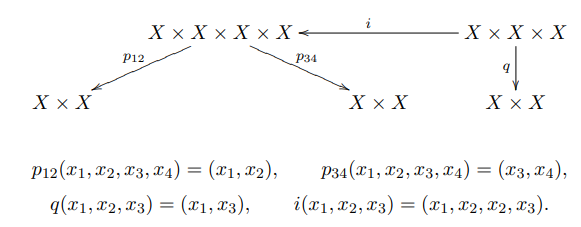
\includegraphics[scale=0.8]{convolution_maps.PNG}
\end{center}

\begin{proof}[Proof of Theorem~\ref{theorem:hecke_basis}]
We'll prove Theorem~\ref{theorem:hecke_basis} by induction. The base cases consist of $w = 1$ and $w = s$ for a simple reflection $s$. We have $\overline{O}_1 = X$, so $\mr{IC}_{\overline{O}_1} \cong \mathbb{C}_{\overline{O}_1}[\delta]$, and $\widehat{\mr{IC}_{\overline{O}_1}} = T_1 = C_1^{\prime}$. $p_1: \overline{O}_s \to X$ is a Zariski fibration with fiber $\overline{X}_s \cong \mathbb{P}^1$, so $\overline{O}_s$ is smooth of dimension $1 + \delta$, and $\mr{IC}_{\overline{O}_s} \cong \mathbb{C}_{\overline{O}_s}[1 + \delta]$. The Schubert stratification gives $\overline{O}_s = O_1 \sqcup O_s$, so $\widehat{h}(\mr{IC}_{\overline{O}_s}) = q^{-1/2}(T_s + T_1) = C_s^{\prime}$. In particular, $\mr{IC}_{\overline{O}_1},\mr{IC}_{\overline{O}_s} \in \mathcal{C}$.

To induct, we'll show that convolution with $\mr{IC}_{\overline{O}_s}$ corresponds to multiplication by $C_s^{\prime}$ in the Hecke algebra.

\begin{lem}\label{lemma:mult_simp}
For $K \in \mathcal{C}$, $\widehat{h}(\mr{IC}_{\overline{O}_s} \star K) = C_s^{\prime}\widehat{h}(K)$. In particular, $\mr{IC}_{\overline{O}_s} \star K \in \mathcal{C}$.
\end{lem}

\begin{proof}
This is proven by a direct computation. We have $$p_{12}^*\mr{IC}_{\overline{O}_s} \cong \mathbb{C}_{\overline{O}_s \times X \times X}[1 + \delta],$$ so $$\mr{IC}_{\overline{O}_s} \star K \cong q_*i^*(p_{34}^*K)|_{\overline{O}_s \times X \times X}[1 + \delta].$$ Let $p = (B,wB)$ be a point of $O_w$. Then $q^{-1}(p) \cap i^{-1}(\overline{O}_s \times X \times X) = \{(B,x,wB)|x \in \overline{X}_s\} \cong \mathbb{P}^1$. Let $Y$ denote this $\mathbb{P}^1$. Then $\mathcal{H}^i(\mr{IC}_{\overline{O}_s} \star K)_p \cong H^{i + \delta + 1}(Y,K|_Y)$. By constructibility on $X \times X$, $K|_Y$ is constructible with respect to $Y = U \sqcup u_0$, where $U \cong \mathbb{C}$ and $u_0$ is a point. Because $U$ is contractible and $K|_U$ is a complex with locally constant cohomology, each $\mathcal{H}^i(K)$ is a constant sheaf, and $K|_U \simeq \bigoplus_i\mathcal{H}^i(K)[-i]$. The decomposition $Y = U \sqcup u_0$ gives us a long exact sequence in compactly supported cohomology $\cdots \to H_c^i(U,K|_U) \to H^i(Y,K|_Y) \to \mathcal{H}^i(K)|_{u_0} \to \cdots$. By parity vanishing, this long exact sequence splices into short exact sequences $0 \to H_c^i(U,K|_U) \to H^i(Y,K|_Y) \to \mathcal{H}^i(K)|_{u_0} \to 0$. Poincar\'{e} duality tells us that $\dim H_c^i(U,K|_U) = \dim H^{i - 2}(U,K|_U) = \dim\mathcal{H}^{i - 2}(U)|_u$ for any $u \in U$. Thus, $h^i(\mr{IC}_{\overline{O}_s} \star K)_w = \dim H^i(Y,K|_Y) = \dim\mathcal{H}^{i - 2}(U)|_u + \dim\mathcal{H}^i(U)|_{u_0}$.

To finish, we must identify which strata of $X \times X$ contain $u$ and $u_0$. If $sw > w$, then $u \in O_{sw}$, and $u_0 \in O_w$, so that $h^i(\mr{IC}_{\overline{O}_s} \star K)_w = h^{i + \delta + 1}(K)|_w + h^{i + \delta - 1}(K)|_{sw}$. If $sw < w$, then $u \in O_w$, and $u_0 \in O_{sw}$, so that $h^i(\mr{IC}_{\overline{O}_s} \star K)_w = h^{i + \delta + 1}(K)|_{sw} + h^{i + \delta - 1}(K)|_w$. This turns out to be the formula for multiplication by $C_s^{\prime}$.

\end{proof}

To finish the proof, we must compute the remaining $\mr{IC}_{\overline{O}_w}$. Unlike the $\overline{O}_s$, $\overline{O}_w$ might not be smooth, so $\mr{IC}_{\overline{O}_w}$ might not just be a shifted constant sheaf. To compute $\mr{IC}_{\overline{O}_w}$, we apply the decomposition theorem to the \textit{Bott-Samelson resolution} $\pi: \widetilde{O}_w \to \overline{O}_w$. For a reduced expression $w = s_1\ldots s_{\ell}$, we define $\widetilde{O}_w \coloneqq \{(B_1,\ldots,B_{\ell + 1}) \in X^{\ell + 1}|(B_i,B_{i + 1}) \in \overline{O}_{s_i}\}$. $\widetilde{O}_w$ is smooth because $\widetilde{O}_w \to \mathbb{P}^1$ is a $(\mathbb{P}^1)^{\ell}$-fibration. $\pi: \widetilde{O}_w \to \overline{O}_w$ is defined by $\pi(B_1,\ldots,B_{\ell + 1}) = (B_1,B_{\ell + 1})$; this is an isomorphism over $O_w$, so it is a resolution of singularities.

By definition, $\pi_*\mathbb{C}_{\widetilde{O}_w}[\delta + \ell] = \mr{IC}_{\overline{O}_{s_1}} \star \cdots \star \mr{IC}_{\overline{O}_{s_{\ell}}}$. Thus, by \Cref{lemma:mult_simp}, $\widehat{h}(\pi_*\mathbb{C}_{\widetilde{O}_w}[\delta + \ell]) = C_{s_1}^{\prime}\cdots C_{s_{\ell}}^{\prime} = q^{-\ell/2}(T_{s_1} + T_1)\cdots(T_{s_{\ell}} + T_1)$. Since $\widetilde{O}_w$ is smooth, $\mathbb{C}_{\widetilde{O}_w}[\delta + \ell] = \mr{IC}_{\widetilde{O}_w}$, and the \textit{decomposition theorem} (which I will not state or explain) states that $\pi_*\mathbb{C}_{\widetilde{O}_w}[\delta + \ell]$ is a direct sum of shifted $\mr{IC}_{\overline{O}_v}$'s: $\pi_*\mathbb{C}_{\widetilde{O}_w}[\delta + \ell] \cong \mr{IC}_{\overline{O}_w} \oplus \bigoplus_{v < w}\bigoplus_i\mr{IC}_{\overline{O}_v} \otimes V_v^i[-i]$ for some finite-dimensional $\mathbb{C}$-vector spaces $V_v^i$. Since $\mr{IC}_{\overline{O}_w}$ is a direct summand of $\pi_*\mathbb{C}_{\widetilde{O}_w}[\delta + \ell] \in \mathcal{C}$, $\mr{IC}_{\overline{O}_w} \in \mathcal{C}$. Applying $\widehat{h}$, we have $C_{s_1}^{\prime}\cdots C_{s_{\ell}}^{\prime} = \widehat{h}(\mr{IC}_{\overline{O}_w}) + \sum_{v < w}F_v(q)\widehat{h}(\mr{IC}_{\overline{O}_v})$, where $F_v(q) = \sum_j(\dim V_v^j)q^{j/2}$. Since $\mathbb{C}_{\widetilde{O}_w}[\delta + \ell]$ is self-dual and $\pi$ is proper, $\mathbb{D}\prescript{p}{}{}\mathcal{H}^i(\pi_*\mathbb{C}_{\widetilde{O}_w}[\delta + \ell]) \cong \mathcal{H}^{-i}(\pi_*\mathbb{C}_{\widetilde{O}_w}[\delta + \ell])$, and $\dim V_v^i = \dim V_v^{-i}$. This implies that $F_v(q) = F_v(q^{-1})$.

By induction on length, we have $\widehat{h}(\mr{IC}_{\overline{O}_w}) = C_{s_1}^{\prime}\cdots C_{s_{\ell}}^{\prime} - \sum_{v < w}P_v(q)C_v^{\prime}$. Since everything on the RHS is self-dual in $\mathcal{H}(W)$, $\widehat{h}(\mr{IC}_{\overline{O}_w})$ must be self-dual. It remains to see that if we write $\widehat{h}(\mr{IC}_{\overline{O}_w}) = q^{-\ell/2}\sum_{v \le w}\widetilde{P}_{v,w}(q)T_v$, then (1) $\widetilde{P}_{v,w}(q) \in \mathbb{Z}[q]$, (2) $\widetilde{P}_{w,w} = 1$, and (3) $\deg\widetilde{P}_{v,w} \le \frac{1}{2}(\ell(w) - \ell(v) - 1)$: \begin{enumerate}[(1)]
\item This follows from the fact that $\mr{IC}_{\overline{O}_w} \in \mathcal{C}$.

\item This follows from the equation $\widehat{h}(\mr{IC}_{\overline{O}_w}) = C_{s_1}^{\prime}\cdots C_{s_{\ell}}^{\prime} - \sum_{v < w}P_v(q)C_v^{\prime}$, as the first term contributes $q^{-\ell/2}T_w$ and no other terms contribute any.

\item This follows from the support condition on $\mr{IC}_{\overline{O}_w}$: $\mathcal{H}^{i - \ell(w)}(\mr{IC}_{\overline{O}_w})_v \cong 0$ if $\dim O_v \ge -(i - \ell(w))$. Since $\dim O_v = \delta + \ell(v)$, this says that $i + \delta \ge \ell(w) - \ell(v)$. Thus, $\deg\widetilde{P}_{v,w}(q) < \frac{1}{2}(\ell(w) - \ell(v))$, as desired.

\end{enumerate}

By the uniqueness of the Kazhdan-Lusztig polynomials, $\widetilde{P}_{v,w} = P_{v,w}$, and $h(\mr{IC}_{\overline{X}_w}) = \widehat{h}(\mr{IC}_{\overline{O}_w}) = C_w^{\prime}$, as desired.

\end{proof}

To finish the proof of the Kazhdan-Lusztig conjecture, for $K \in \Perv(X)_W$, we define $\chi^W(K) \coloneqq \sum_v\sum_i(-1)^i\mathcal{H}^i(K)_vv \in \mathbb{Z}[W]$. By parity vanishing (in particular, $\mathcal{H}^i(\mr{IC}_{\overline{X}_w}) \ne 0$ only when $i \equiv \ell(w) \pmod{2}$), 
\[ \chi^W(\mr{IC}_{\overline{X}_w}) = \sum_v\sum_i(-1)^ih^i(\mr{IC}_{\overline{X}_w})_vv = \sum_v(-1)^{\ell(w)}\sum_ih^i(\mr{IC}_{\overline{X}_w})v = \sum_v(-1)^{\ell(w)}P_{v,w}(1)v. \] We have $\chi^W(\mathbb{C}_{X_w}) = (-1)^{\ell(w)}w$. From these computations, we see that $\chi^W: K(\Perv(X)_W) \to \mathbb{Z}[W]$ is an isomorphism of $\mathbb{Z}$-modules. Since $\chi^W(\mr{IC}_{\overline{X}_w}) = \sum_v(-1)^{\ell(w) - \ell(v)}P_{v,w}(1)\chi^W(\mathbb{C}_{X_v})$, we see that $[\mr{IC}_{\overline{X}_w}] = \sum_v(-1)^{\ell(w) - \ell(v)}P_{v,w}(1)[\mathbb{C}_{X_v}]$ in $K(\Perv(X)_W)$, which is exactly what we want.


\end{document}
